%%%%%%%%%%%%%%%%%%%% book.tex %%%%%%%%%%%%%%%%%%%%%%%%%%%%%
%
% sample root file for the chapters of your "monograph"
%
% Use this file as a template for your own input.
%
%%%%%%%%%%%%%%%% Springer-Verlag %%%%%%%%%%%%%%%%%%%%%%%%%%


% RECOMMENDED %%%%%%%%%%%%%%%%%%%%%%%%%%%%%%%%%%%%%%%%%%%%%%%%%%%
\documentclass[graybox,envcountchap,sectrefs]{svmono}

% choose options for [] as required from the list
% in the Reference Guide

\usepackage{mathptmx}
\usepackage{helvet}
\usepackage{courier}
%
\usepackage{type1cm}         

\usepackage{makeidx}         % allows index generation
\usepackage[pdftex]{graphicx}        % standard LaTeX graphics tool
                             % when including figure files
\usepackage{multicol}        % used for the two-column index
\usepackage[bottom]{footmisc}% places footnotes at page bottom

% see the list of further useful packages
% in the Reference Guide

\makeindex             % used for the subject index
                       % please use the style svind.ist with
                       % your makeindex program

%%%%%%%%%%%%%%%%%%%%%%%%%%%%%%%%%%%%%%%%%%%%%%%%%%%%%%%%%%%%%%%%%%%%%

\begin{document}

\author{Author name(s)}
\title{Book title}
\subtitle{-- Monograph --}
\maketitle

\frontmatter%%%%%%%%%%%%%%%%%%%%%%%%%%%%%%%%%%%%%%%%%%%%%%%%%%%%%%


%%%%%%%%%%%%%%%%%%%%%%% dedic.tex %%%%%%%%%%%%%%%%%%%%%%%%%%%%%%%%%
%
% sample dedication
%
% Use this file as a template for your own input.
%
%%%%%%%%%%%%%%%%%%%%%%%% Springer %%%%%%%%%%%%%%%%%%%%%%%%%%

\begin{dedication}
Use the template \emph{dedic.tex} together with the Springer document class SVMono for monograph-type books or SVMult for contributed volumes to style a quotation or a dedication\index{dedication} at the very beginning of your book in the Springer layout
\end{dedication}





%%%%%%%%%%%%%%%%%%%%%%foreword.tex%%%%%%%%%%%%%%%%%%%%%%%%%%%%%%%%%
% sample foreword
%
% Use this file as a template for your own input.
%
%%%%%%%%%%%%%%%%%%%%%%%% Springer %%%%%%%%%%%%%%%%%%%%%%%%%%

\foreword

%% Please have the foreword written here
Use the template \textit{foreword.tex} together with the Springer document class SVMono (monograph-type books) or SVMult (edited books) to style your foreword\index{foreword} in the Springer layout. 

The foreword covers introductory remarks preceding the text of a book that are written by a \textit{person other than the author or editor} of the book. If applicable, the foreword precedes the preface which is written by the author or editor of the book.


\vspace{\baselineskip}
\begin{flushright}\noindent
Place, month year\hfill {\it Firstname  Surname}\\
\end{flushright}



%%%%%%%%%%%%%%%%%%%%%%preface.tex%%%%%%%%%%%%%%%%%%%%%%%%%%%%%%%%%%%%%%%%%
% sample preface
%
% Use this file as a template for your own input.
%
%%%%%%%%%%%%%%%%%%%%%%%% Springer %%%%%%%%%%%%%%%%%%%%%%%%%%

\preface

%% Please write your preface here
Use the template \emph{preface.tex} together with the Springer document class SVMono (monograph-type books) or SVMult (edited books) to style your preface in the Springer layout.

A preface\index{preface} is a book's preliminary statement, usually written by the \textit{author or editor} of a work, which states its origin, scope, purpose, plan, and intended audience, and which sometimes includes afterthoughts and acknowledgments of assistance. 

When written by a person other than the author, it is called a foreword. The preface or foreword is distinct from the introduction, which deals with the subject of the work.

Customarily \textit{acknowledgments} are included as last part of the preface.
 

\vspace{\baselineskip}
\begin{flushright}\noindent
Place(s),\hfill {\it Firstname  Surname}\\
month year\hfill {\it Firstname  Surname}\\
\end{flushright}



%%%%%%%%%%%%%%%%%%%%%%acknow.tex%%%%%%%%%%%%%%%%%%%%%%%%%%%%%%%%%%%%%%%%%
% sample acknowledgement chapter
%
% Use this file as a template for your own input.
%
%%%%%%%%%%%%%%%%%%%%%%%% Springer %%%%%%%%%%%%%%%%%%%%%%%%%%

\extrachap{Acknowledgements}

Use the template \emph{acknow.tex} together with the Springer document class SVMono (monograph-type books) or SVMult (edited books) if you prefer to set your acknowledgement section as a separate chapter instead of including it as last part of your preface.



\tableofcontents

%%%%%%%%%%%%%%%%%%%%%%acronym.tex%%%%%%%%%%%%%%%%%%%%%%%%%%%%%%%%%%%%%%%%%
% sample list of acronyms
%
% Use this file as a template for your own input.
%
%%%%%%%%%%%%%%%%%%%%%%%% Springer %%%%%%%%%%%%%%%%%%%%%%%%%%

\extrachap{Acronyms}

Use the template \emph{acronym.tex} together with the Springer document class SVMono (monograph-type books) or SVMult (edited books) to style your list(s) of abbreviations or symbols in the Springer layout.

Lists of abbreviations\index{acronyms, list of}, symbols\index{symbols, list of} and the like are easily formatted with the help of the Springer-enhanced \verb|description| environment.

\begin{description}[CABR]
\item[ABC]{Spelled-out abbreviation and definition}
\item[BABI]{Spelled-out abbreviation and definition}
\item[CABR]{Spelled-out abbreviation and definition}
\end{description}


\mainmatter%%%%%%%%%%%%%%%%%%%%%%%%%%%%%%%%%%%%%%%%%%%%%%%%%%%%%%%
%%%%%%%%%%%%%%%%%%%%%part.tex%%%%%%%%%%%%%%%%%%%%%%%%%%%%%%%%%%
% 
% sample part title
%
% Use this file as a template for your own input.
%
%%%%%%%%%%%%%%%%%%%%%%%% Springer %%%%%%%%%%%%%%%%%%%%%%%%%%

\begin{partbacktext}
\part{Part Title}
\noindent Use the template \emph{part.tex} together with the Springer document class SVMono (monograph-type books) or SVMult (edited books) to style your part title page and, if desired, a short introductory text (maximum one page) on its verso page in the Springer layout.

\end{partbacktext}
%%%%%%%%%%%%%%%%%%%%% chapter.tex %%%%%%%%%%%%%%%%%%%%%%%%%%%%%%%%%
%
% sample chapter
%
% Use this file as a template for your own input.
%
%%%%%%%%%%%%%%%%%%%%%%%% Springer-Verlag %%%%%%%%%%%%%%%%%%%%%%%%%%
%\motto{Use the template \emph{chapter.tex} to style the various elements of your chapter content.}
\chapter{Introduction}
\label{introduction} % Always give a unique label
% use \chaptermark{}
% to alter or adjust the chapter heading in the running head

\abstract*{As one of the key areas that appeals directly to the majority of the human race, Virtual Reality is receiving a high level of attention at present. Despite this, there is still much space for growth within the field for navigation frameworks. In this chapter, We introduce our framework by defining the problem we seek to address. Details regarding importance of this project and the necessary background details, including relevant details from industry projects, are succinctly summarized. An analysis of existing industrial trends pertaining to VR included as well. The scope of the project is defined along with the expected outcomes. Research outcomes expected from this project are described in considerable depth with the hope of providing a clear outline of the scientific contribution of the project.}

\abstract{As one of the key areas that appeals directly to the majority of the human race, Virtual Reality is receiving a high level of attention at present. Despite this, there is still much space for growth within the field for navigation frameworks. In this chapter, We introduce our framework by defining the problem we seek to address. Details regarding importance of this project and the necessary background details, including relevant details from industry projects, are succinctly summarized. An analysis of existing industrial trends pertaining to VR included as well. The scope of the project is defined along with the expected outcomes. Research outcomes expected from this project are described in considerable depth with the hope of providing a clear outline of the scientific contribution of the project.}

\section{Problem Background}
\label{sec:1}

The concept of Virtual Reality first emerged during 1950s and experiencing Virtual Reality using a head mounted display system wasn?t introduced during late 1960s. With the advances in the field of generation of 3D content and image processing, this topic caught the interest of many and the recent release of Oculus RIFT, SamsaungVR gear and especially Google Cardboard as an inexpensive alternative, the field is once again in the limelight. However generating content for virtual reality applications still remains to be a technically challenging and expensive task. Thus Virtual Reality is still a cutting edge technology with a great deal of unexplored potential.

Currently VR technologies are mostly used for games, to create an immersive experience within a computer generated environment. The few uses of real world content account to the fact that the content generation process requires dedicated hardware and proprietary software, but even with that the generated environment is immensely restrictive. Therefore mass scale applications utilizing VR technologies are almost non-existent.

However, the use of Virtual Reality in the fields of Medicine, Education, and Media etc... Is being explored and researched by scholars and it has emerged as a very promising technology. Hence, VR could be stated to be one of the timeliest areas for research and development in.

\section{Importance of the Problem}
\label{intro_sec:2}
% Always give a unique label
% and use \ref{<label>} for cross-references
% and \cite{<label>} for bibliographic references
% use \sectionmark{}
% to alter or adjust the section heading in the running head

\subsection{Growth of Industry}
\label{intro_subsec:2_1}

Virtual Reality is becoming the future of immersion for computer generated imagery. As the following business insider graph predicts, the shift to virtual reality is increasing drastically.

\begin{figure}[htbp]
\begin{center}
\includegraphics[width=\textwidth]{Figures/1.png}
\caption{Global Virtual Reality Head-Mounted Display Shipments \cite{1}}
\label{fig1_1}
\end{center}
\end{figure}


With the increase of availability of the virtual reality hardware, the market potential of VR has a significant importance. The graph below shows the percentage of income from VR in different areas.

Therefore the greater part of VR revenue will depend on the software solutions available to exploit the shift to VR. This is evident by many start-ups forming to take advantage of this market niche such as, Jaunt VR \cite{4}, Vahana VR \cite{5}, Samsung LiveLife \cite{6}, HP ZVR \cite{7}.

Not only start-ups, all the big players in the industry have started investing heavily on virtual reality technologies. This is evident through projects such as Google Cardboard project \cite{2} which aims to make virtual reality accessible at a low cost, Microsoft?s Hololense \cite{8}. Even Facebook has joined up the VR hype by acquiring the Oculus which was the leading virtual reality headband producer at the time.

\begin{figure}[htbp]
\begin{center}
\includegraphics[width=\textwidth]{Figures/2.png}
\caption{Augmented and Virtual Reality To Hit \$150 Billion \cite{3}}
\label{fig1_2}
\end{center}
\end{figure}

With these new trends a significant reduction of cost can be seen for Virtual reality hardware. Unlike the old days, anyone who owns a smartphone may convert it to a virtual reality head band with the google cardboard at a very low cost. With this drastic reduction in cost virtual reality is accessible by any person. However the content creation remains a high costly process requiring specialized equipment. This is a barrier this project aims to eliminate.

\subsection{Applications Utilizing VR}
\label{intro_subsec:2_2}

This new trend in virtual reality has helped in many professions and fields. For an example in the medical industry \cite{9}. The special use cases in surgery is discussed in this paper \cite{10}. The use of VR in therapy and rehabilitation is another use case for this technology. 

Man, mind, and machine: the past and future of virtual reality simulation in neurologic surgery discusses the use of VR in neurologic surgery \cite{11}.

Other than the medical field there are uses in Virtual reality technologies in education, training and marketing areas as well which are elaborated in Immersive training systems: Virtual Reality and Education and Training \cite{12} and  The Effects of Virtual Reality on Consumer Learning (Marketing) \cite{13}.

\subsection{Space for Improvement}
\label{intro_subsec:2_3}

The project will focus greatly on the underlying algorithms for creating content as well as rendering content. In order to successfully use low cost smartphones and cameras, and give an immersive experience through virtual reality these algorithms need to be optimised to use the least amount of resources.

Thus by analysing image stitching, video stitching and rendering algorithms and optimising them for the use on mobile phones with their inherent limitations in computational power and memory, the project will have huge impact on making VR technology widely available.

This contribution of the project will give the required core software backing to complete the transition of virtual reality from unaffordable to affordable.

\section{Scope of the Project}
\label{intro_sec:3}

The project work plans to deliver a significant contribution to the scientific research in the fields in Computer Vision, Image Processing, Virtual Reality, and other related fields.

Major contributions from the project has been identified as the following:

\begin{itemize}
\item{An evaluation of Image Stitching Algorithms}
\item{A mathematical model for generating intermediate spheres}
\item{An optimization strategy for streaming immersive VR over a network}
\item{A Scene Description Language for representing Navigable VR environments}
\item{Intuitive gesture system based on a Machine Learning Algorithm}
\item{A four-camera rig which aligns itself with the compass direction}
\end{itemize}

\subsection{An Evaluation of Image Stitching Algorithms}
\label{intro_subsec:3_1}

The first stage of the project would be to analyse existing algorithms for Image stitching algorithms. After conducting a thorough literature survey, several Image stitching algorithms, including the following will be chosen for testing.

\begin{itemize}
\item{Fast panorama stitching for high-quality panoramic images on mobile phones \cite{14}}
\item{Automatic Panorama Image Stitching using Invariant Features \cite{15}}
\item{Video Stitch Algorithm Based on Dynamic Foreground Extraction \cite{16}}
\item{Efficient Video Panoramic Image Stitching Based on an Improved Selection of Harris Corners and a Multiple-Constraint Corner Matching \cite{17}}
\item{Stitching Video from Webcams}
\end{itemize}

A testing framework will be developed to assess the qualitative aspects as well as quantitative aspects of the each algorithm. The colour correction and the structure of the stitched image would be taken into account for this testing.

\paragraph{Expected Outcomes}
\begin{itemize}
\item{Implementation of image stitching techniques described in the selected research papers.}
\item{Testing framework for image stitching.}
\item{Evaluation method for image stitching algorithms capturing both qualitative and quantitative aspects.}
\end{itemize}

\paragraph{Deliverables}
\begin{itemize}
\item{Research paper evaluating selected image stitching algorithms.}
\end{itemize}
The paper will present the testing framework and the test results, and differentiate each algorithm and identify their strong points and weaknesses which will help to choose the best algorithm for the project.

\subsection{Image Sphere}
\label{intro_subsec:3_2}

The next phase of the project is to create the image sphere using a set of images. Using the selected image stitching algorithm from the previous phase a panorama of the full 360 x 360 degree images will be created. 

In order to use this stitched panorama it will be projected onto a sphere, several methods for projecting a 2D panorama into a sphere will be considered along with the representation of these for rendering.

\paragraph{Expected Outcomes}
\begin{itemize}
\item{Storing image spheres in a portable format.}
\item{Rendering image spheres in google cardboard app.}
\end{itemize}

\paragraph{Deliverables}
\begin{itemize}
\item{PoC system for stitching and viewing 360 images}
\end{itemize}

\subsection{Navigation in a Static Environment}
\label{intro_subsec:3_3}

After the image stitching and projection on a sphere is complete we would look at giving the user a more immersive experience by making it possible to navigate through the environment. This would be done by creating image spheres as the point of view changes using the available image sphere data.

Our target will be to adopt this technique and improve it keeping in mind the constraints imposed when we use smartphones as the device to run our application.

Moreover, in order to make the traversal process less time consuming, an environment map will be pre-generated, and stored in a Scene Description Language (SDL) embedded into the image spheres.

\paragraph{Expected Outcomes}
\begin{itemize}
\item{Navigation in-between Static 360$^{\circ}$$\times$360$^{\circ}$ panoramic images.}
\end{itemize}

\paragraph{Deliverables}
\begin{itemize}
\item{A Scene Description Language (SDL) for navigation in static panoramic image environments.}
\item{A mathematical model for intermediate sphere generation.}
\item{Research paper on the navigation technique and final outcome of the project.}
\end{itemize}

\subsection{Immersive and Intuitive Gesture-based Navigation}
\label{intro_subsec:3_4}

When the environment itself is fully navigable, and the user is able to experience the immersive reality with minimal restrictions, the remaining question will be the method of navigation.

Walking around is not practical as physical movements while wearing a VR headgear is bound to be dangerous to the person. A button based input system is unsophisticated as it will be ruining the immersive experience of the user. Hence as a solution we would explore the possibilities of implementing an intuitive gesture, which is practical and supportive to the illusion of immersiveness.

\paragraph{Expected Outcomes}
\begin{itemize}
\item{The user is able to freely navigate within the immersive environment.}
\end{itemize}

\paragraph{Deliverables}
\begin{itemize}
\item{An intuitive gesture input system for navigation inside a virtual environment}
\item{Research paper on the intuitive gesture recognition system}
\end{itemize}

\subsection{Optimization Strategy for Streaming VR Content}
\label{intro_subsec:3_5}

By nature, VR content requires a lot of information. Thus, streaming VR content over a network necessitates more data. But, for a user immersed in a virtual world, all the details are not important, as the Field of View of is quite narrow. However, just streaming the data attached to the viewpoint is not feasible as a user making a sudden movement will require different areas of vision.

Our research work aims to find a suitable mechanism to allow the users to have an immersive experience while making sure the data flow over the network is minimal. Possible solutions include, differentiating the quality of streamed data, and predicting user movements, etc..

\paragraph{Expected Outcomes}
\begin{itemize}
\item{The system is able to stream VR data with minimal data consumption.}
\end{itemize}

\paragraph{Deliverables}
\begin{itemize}
\item{An optimization algorithm for streaming VR content over a network.}
\end{itemize}

\subsection{Multi-camera Rig for Panoramic Image Capture}
\label{intro_subsec:3_6}

In order to generate panoramas, it is not practical to acquire individual photos and send them into a stitching process to obtain it. Thus, one of the objectives in this research work is to create a multi camera rig, specially designed to capture panoramas, along with location data for environment generation \cite{18}. 

Also, the camera rig needs to be equipped with a self-adjusting feature to align itself to the same compass direction for taking panoramic photos in the same series. This is in order to make aligning the panoramas without further calculations.

\paragraph{Expected Outcomes}
\begin{itemize}
\item{The user is able to capture photos from a camera rig, without worrying about technical details.}
\end{itemize}

\paragraph{Deliverables}
\begin{itemize}
\item{A physical four-camera rig, self-adjusting to the same compass direction.}
\end{itemize}

\section{Coverage of Research Areas}
\label{intro_sec:4}

As a project that involves mapping real world scenarios to virtual environments and allowing visualization using Virtual Reality, this project covers several key research areas in computer science.

Primary among these are,
\begin{enumerate}
\item{Image Processing}
\item{Computer Vision}
\item{Computer Graphics}
\item{Human Computer Interaction}
\item{Machine Learning}
\end{enumerate}

\paragraph{Image Processing}
%\label{intro_subsec:4_1}
As a framework for creating VR content using image input, the pre-processing steps used in images at various steps form a crucial part of the system. These include grey scaling, applying various filters, edge detection and colour correction.

\paragraph{Computer Vision}
%\label{intro_subsec:4_2}
In creating a panoramic image using individual images, image stitching is especially important. In performing stitching, feature extraction and correlation form the very basis of correlating matching parts of separate images together.

\paragraph{Computer Graphics}
%\label{intro_subsec:4_3}
Projecting the stitched panorama into a sphere and additionally providing an intuitive visualization of the sphere using a game engine falls under the category of Computer Graphics.

\paragraph{Human Computer Interaction}
%\label{intro_subsec:4_4}
Using a VR headset for navigation is not inherently intuitive. As the interactivity of the scene is increased, providing an intuitive navigation framework becomes harder. Suggesting a seamless navigation method which provides a smooth experience for the viewer is very important to the overall goal of ensuring immersiveness.

\paragraph{Machine Learning}
%\label{intro_subsec:4_5}
Navigating using gestures provides its own challenge of recognizing said gestures. A machine learning based approach is considered in this regard so as to ensure the maximum accuracy along with very high responsiveness.

%%%%%%%%%%%%%%%%%%%%% chapter.tex %%%%%%%%%%%%%%%%%%%%%%%%%%%%%%%%%
%
% sample chapter
%
% Use this file as a template for your own input.
%
%%%%%%%%%%%%%%%%%%%%%%%% Springer-Verlag %%%%%%%%%%%%%%%%%%%%%%%%%%
%\motto{Use the template \emph{chapter.tex} to style the various elements of your chapter content.}
\chapter{Literature Review}
\label{lit_review} % Always give a unique label
% use \chaptermark{}
% to alter or adjust the chapter heading in the running head

%\abstract*{Each chapter should be preceded by an abstract (10--15 lines long) that summarizes the content. The abstract will appear \textit{online} at \url{www.SpringerLink.com} and be available with unrestricted access. This allows unregistered users to read the abstract as a teaser for the complete chapter. As a general rule the abstracts will not appear in the printed version of your book unless it is the style of your particular book or that of the series to which your book belongs.
%Please use the 'starred' version of the new Springer \texttt{abstract} command for typesetting the text of the online abstracts (cf. source file of this chapter template \texttt{abstract}) and include them with the source files of your manuscript. Use the plain \texttt{abstract} command if the abstract is also to appear in the printed version of the book.}

\abstract{While Virtual Reality is the main focus in our research work, we peruse many concepts and novel ideas from a number of different fields. This chapter provides a review of techniques we have considered from a number of fields such as Computer Vision, Image Processing, Machine Learning, Optimization and Virtual Reality. Under Computer Vision and Image Processing, Image stitching algorithms and evaluation techniques have been explored in depth. Pattern recognition and Machine Learning techniques, particularly pertaining to gesture recognition using accelerometer and gyro sensor data, have been thoroughly reviewed. Intermediate scene interpolation and scene description languages have also been reviewed, towards achieving the goal of creating a freely navigable environment.}

\section{Image Stitching}
\label{lit_sec:1}
In order to find the most suited image stitching algorithm for the current task multiple existing image stitching algorithms were taken into account, out of these four image stitching algorithms were selected for implementation and testing.

\subsection{Feature Detection}
\label{lit_sub_sec:1_1}
% Always give a unique label
% and use \ref{<label>} for cross-references
% and \cite{<label>} for bibliographic references
% use \sectionmark{}
% to alter or adjust the section heading in the running head
Feature detection is an integral part of image stitching. Two main methods used in the feature detection are SIFT and SURF.

In any application which needs images registration/alignment the main steps required are feature detection, feature matching, deriving a transform function and reconstructing images based on the transform function. For a successful image registration many methods have been used for feature detection, two of the main such methods are:
\begin{itemize}
\item SIFT: Scale Invariant Feature Transform
\item SURF: Speed Up Robust Features
\end{itemize}

Both these are scale and rotation invariant detector and descriptor algorithms \cite{panchal2013}.

\subsubsection{SIFT Algorithm}
Sift algorithm was introduced in "Distinctive Image Features from Scale-Invariant Key points" by Lowe et al. 2004 \cite{Lowe2004}.

The SIFT algorithm flow is as follows:

\begin{figure}[htbp]
\sidecaption
\includegraphics[width=\textwidth]{3.png}
\caption{SIFT Algorithm Flow}
\label{Fig_2_SIFT_flow}       % Give a unique label
\end{figure}

An overview of the extrema detection method used in SIFT is as follows. This method enables detection of points as well as blobs.

\begin{figure}[htbp]
\sidecaption
\includegraphics[width=\textwidth]{4.png}
\caption{Gaussian method}
\label{Fig_2_Gaussian_method}       % Give a unique label
\end{figure}

SIFT uses $\gamma$ termed scale with the coordinates of a point to define the scale space function $L(x, y, \gamma)$ which produced from the convolution of a variable-scale Gaussian. As the scale increases the image get blurred and smoother.

An interest point in SIFT is identified when a given point is a local extrema of twenty six pixels around it, when considered with the images of the scale lower and higher to it. Taylor series approximation can be used to identify extrema. The size of the blob detected corresponds to the scale it is detected in.

\begin{figure}[htbp]
\sidecaption
\includegraphics[scale=1]{5.png}
\caption{Blob Size vs Scale}
\label{Fig_2_blob_scale}       % Give a unique label
\end{figure}

Using the Hessian matrix the edge responses are eliminated. Then the image is subsampled into a different octave and the similar scale space detection is carried out. This enables to identify the stable key points from the detected set. To achieve rotation invariance a weighted direction histogram is created for 4$\times$4 neighbourhood of the interest point into 36 bins. This serves as the local descriptor for an image.

\begin{figure}[htbp]
\sidecaption
\includegraphics[width=\textwidth]{6.png}
\caption{Extracting key point descriptors from image gradients}
\label{Fig_2_key_point}       % Give a unique label
\end{figure}

\subsubsection{SURF Algorithm}
SURF was introduced in the paper "SURF: Speeded UP Robust Features" by Herbert et al. in 2006 \cite{Bay2006}. It uses the same flow as SIFT, but utilizes a different scheme to achieve that. Thus results in a faster and better results. We will discuss the SURF algorithm in two places, Detection of features, and generating the descriptor for each feature.

\paragraph*{\textbf{Detection of Features}}
The goal is to detect interesting points in the image, and these points to be detected always, regardless of the viewpoint. A Laplacian \cite{Mikolajczyk2001} of Gaussian is approximated with a Box Filter in the SURF algorithm.

SURF uses an integral image, denoted as $I(x)$, where,
\textbf{eqn}

\begin{figure}[htbp]
\sidecaption
\includegraphics[scale=0.4]{7.png}
\caption{Integral Image}
\label{Fig_2_integral}       % Give a unique label
\end{figure}

Thus, to calculate the response in a particular rectangular area of the image, only four - lookups are needed. Both SIFT and SURF divides the scale space $(x, y, s)$, a mapping of $x, y$ coordinates and scale, into octaves and levels. While SIFT downscales the image, SURF uses increasingly larger files. This allows SURF to calculate responses with arbitrarily large kernels.

\begin{figure}[htbp]
\sidecaption
\includegraphics[scale=1]{8.png}
\caption{Octaves and Levels}
\label{Fig_2_octaves}       % Give a unique label
\end{figure}

\begin{figure}[htbp]
\sidecaption
\includegraphics[scale=1]{9.png}
\caption{SIFT on left; SURF on right}
\label{Fig_2_sift_surf}       % Give a unique label
\end{figure}

Because it is being scaled up, each kernel need to have an uneven size to have a central pixel. Each lobe, needs to have the same size. The SURF paper discusses this and comes up with a fixed division of scale space into levels and octaves.

\begin{figure}[htbp]
\sidecaption
\includegraphics[scale=1]{10.png}
\caption{Kernels and Lobes}
\label{Fig_2_kernals}       % Give a unique label
\end{figure}

With this model, extrema can be found out, and they are detected as points of interests \cite{Pedersen2011}.

\paragraph*{\textbf{Description of Features}}

The purpose of a descriptor is to provide a unique and robust description of a detected feature. It is usually based on the surrounding of the interest point.

Features need to be rotational and scale invariant as well, for most purposes. But, for the purposes of a panoramic stitching algorithm, rotational invariance is not needed, as the images are expected to be of the same orientation. Because of this, a special adaptation of this called Upright SURF (U-SURF) can be used. U-SURF works for rotations +/- 15 degrees.

The SIFT and SURF uses distinct ways to assign descriptors. A descriptor based on Haar wavelet response are efficiently calculated in SIFT \cite{Lowe2004}.

A unique vector is generated by using wavelet responses. Considering wavelet responses in the $x$ and $y$ directions as $d_x$ and $d_y$ ,

\begin{align}
\label{eqn:eq1}
\begin{split}
\[
v\ =\ \left\{dx,\ \left\vert{}dx\right\vert{},\ dy,\
\left\vert{}dy\right\vert{}\right\}
\]
\end{split}
\end{align}

This vector, calculated for 16 sub areas in the interest region is concatenated to get the descriptor. Finally, it is normalized, to achieve invariance to contrast variances.This 16$\times$4 descriptor is a 64 dimensional one, and SURF also supports an extended 128 dimensional descriptor, for cases requiring a higher distinctiveness in its features.

\begin{figure}[htbp]
\sidecaption
\includegraphics[scale=1]{11.png}
\caption{Sub areas in a wavelet}
\label{Fig_2_sub_areas}       % Give a unique label
\end{figure}

\subsubsection{Matching Features}
Once the descriptors are calculated, matching two features is just a matter of calculating whether the distance between the two descriptor vectors are sufficiently small, for them to be corresponding features.
Also, in SURF, the Laplassian (Trace of the Hessian Matrix) is calculated, and depending on its sign (+/-) it is decided whether they can be matched or not. This saves a lot of computation, as the sign can decide whether the selected point is a light blob inside a dark background, or a dark blob in a light background.

\begin{figure}[htbp]
\sidecaption
\includegraphics[width=\textwidth]{12.png}
\caption{Preliminary eliminations for Matching in SURF}
\label{Fig_2_matching}       % Give a unique label
\end{figure}

\subsection{Brown and Lowe Method}
The work by Brown and Lowe \cite{Brown2006} discusses an algorithm on multi-image matching, stitching and recognition of correct images while filtering noise images. The approach is targeted at 2D or multi-row stitching of images.

Use of invariant features enables reliable matching of panoramic image sequences despite,
\begin{enumerate}
\item Rotation
\item Zoom
\item Illumination change
\end{enumerate}

Specifying the problem as a multi-image matching problem enables automatic discovery of matching relationships between the images. At the end, seamless output panoramas are rendered using multi-band blending.

\subsubsection{Feature Matching}
SIFT features are extracted and matched between all the images \cite{Lowe99}. As SIFT features are invariant under rotation and scale changes, the algorithm can handle images with varying orientation and zoom.

It is assumed that the camera rotates about its optical centre. Each camera rotation is parametrized by
\begin{enumerate}
\item Rotational vector, $\theta{}\ =\ \left[{\theta{}}_1,{\ \theta{}}_2,\ \ {\theta{}}_3\right]$
\item Focal length, $f$
\end{enumerate}

A pairwise homography is defined as,
\begin{align}
\label{eqn:eq2}
\begin{split}
\[
u_i\ =\ H_{ij}u_j
\]
\end{split}
\end{align}

where, 
\begin{align}
\label{eqn:eq1}
\begin{split}
\[
H_{ij}=K_iR_iR_j^TK_j^{-1}
\]
\end{split}
\end{align}
	
$K_i$ is a 4 parameter model defined on the focal lengths.
$R_i$ is an exponential representation of the rotational vector.

\subsubsection{Image Matching}
The main purpose of this is to find the matching images with overlapping regions. If we match each image with all other images this will be in the quadratic order regarding the number of images. To reduce this images are matched with a constant number of images with the highest number of feature matchers making the complexity order 1.

First RANSAC \cite{Fischler81} is used to select a set of inliers to generate homography between images, and later a probabilistic model is used to verify these matches.

\subsubsection{Bundle Adjustment}
Bundle adjustment \cite{Triggs99} is done to minimise accumulated errors which would be created due to concatenation of pairwise homography (stitching by pairs). The objective function used is a sum squared projection error. Each feature is projected to all the images that match and the error is minimized with respect to the camera parameters. 

\subsubsection{Further enhancements}
Some further enhancements are also discussed. These are listed below. 
\begin{itemize}
\item Automatic Panorama Straightening
\item Gain Compensation
\item Multi-Band Blending
\end{itemize}

The OpenCV \cite{openCV} Image stitching pipeline uses the method given in this paper in its pipeline.

\subsection{Fast Panorama Stitching}
The method presented by Xiong et al. requires little memory and yields relatively faster results. 
In order to stitch images the overlap is needed to be calculated. The method taken for this is described in "Viewfinder Alignment" by Adams et al. \cite{Adams2008}.

\subsubsection{Viewfinder Alignment}
The first step is computing a digest of the image which includes:
\begin{itemize}
\item An integral projection of gradients along four directions. (Edges)
\item Strongest k (=32) Corners on the image.
\end{itemize}

After creating two digests for the adjacent images, the next part is to align them, using only the information available in the digests.
The linear alignment process requires the edges and edge alignment, while the corners are used to calculate a confidence measurement in the aligned image as well as to compute scale and rotational transforms.

\paragraph*{\textbf{Edges and Edge Detection}}
Edges of an image are portions of the image, where there is a sudden change in the visual features. Edge detection algorithms make use of these sharp changes to identify the edges.
To detect the edges, the image is differentiated along an axis. Then the squared value is selected to compensate for negative values. The differentiation technique is not specified in the paper, but we have used the following filters to differentiate along the four major axes (horizontal - x, vertical - y, positive diagonal - u, negative diagonal - v).

\begin{table}[h]
\centering
\begin{tabular}{|p{26pt}|p{26pt}|p{26pt}|}
\hline
\parbox{26pt}{\centering 
+1
} & \parbox{26pt}{\centering 
0
} & \parbox{26pt}{\centering 
-1
} \\
\hline
\parbox{26pt}{\centering 
+2
} & \parbox{26pt}{\centering 
0
} & \parbox{26pt}{\centering 
-2
} \\
\hline
\parbox{26pt}{\centering 
+1
} & \parbox{26pt}{\centering 
0
} & \parbox{26pt}{\centering 
-1
} \\
\hline
\end{tabular}
\\
\caption{Horizantol Axis}
\label{tbl_ha}
\end{table}

\begin{table}[h]
\centering
\begin{tabular}{|p{26pt}|p{26pt}|p{26pt}|}
\hline
\parbox{26pt}{\centering 
+1
} & \parbox{26pt}{\centering 
+2
} & \parbox{26pt}{\centering 
+1
} \\
\hline
\parbox{26pt}{\centering 
0
} & \parbox{26pt}{\centering 
0
} & \parbox{26pt}{\centering 
0
} \\
\hline
\parbox{26pt}{\centering 
-1
} & \parbox{26pt}{\centering 
-2
} & \parbox{26pt}{\centering 
-1
} \\
\hline
\end{tabular}
\\
\caption{Vertical Axis}
\label{tbl_va}
\end{table}

\begin{table}[h]
\centering
\begin{tabular}{|p{26pt}|p{26pt}|p{26pt}|}
\hline
\parbox{26pt}{\centering 
+2
} & \parbox{26pt}{\centering 
+1
} & \parbox{26pt}{\centering 
0
} \\
\hline
\parbox{26pt}{\centering 
+1
} & \parbox{26pt}{\centering 
0
} & \parbox{26pt}{\centering 
-1
} \\
\hline
\parbox{26pt}{\centering 
0
} & \parbox{26pt}{\centering 
-1
} & \parbox{26pt}{\centering 
-2
} \\
\hline
\end{tabular}
\\
\caption{Negative Diagonal}
\label{tbl_nd}
\end{table}

\begin{table}[h]
\centering
\begin{tabular}{|p{26pt}|p{26pt}|p{26pt}|}
\hline
\parbox{26pt}{\centering 
0
} & \parbox{26pt}{\centering 
+1
} & \parbox{26pt}{\centering 
+2
} \\
\hline
\parbox{26pt}{\centering 
-1
} & \parbox{26pt}{\centering 
0
} & \parbox{26pt}{\centering 
+1
} \\
\hline
\parbox{26pt}{\centering 
-2
} & \parbox{26pt}{\centering 
-1
} & \parbox{26pt}{\centering 
0
} \\
\hline
\end{tabular}
\\
\caption{Positive Diagonal}
\label{tbl_pd}
\end{table}

After differentiating along each axis, the differentiated images are integrated along the perpendicular direction (Integral projection) to obtain a graphical digest. The two digests for the images to be stitched along the horizontal axis is shown below:

\textbf{image group}
\begin{figure}[htbp]
\sidecaption
\includegraphics[scale=1]{13.png}
\caption{Integral Projection for the Left Image}
\label{Fig_2_left_img}       % Give a unique label
\end{figure}

\begin{figure}[htbp]
\sidecaption
\includegraphics[scale=1]{14.png}
\caption{Integral Projection for the Right Image.}
\label{Fig_2_right_img}       % Give a unique label
\end{figure}

\paragraph*{\textbf{Edge Alignment}}
Once the two digests are obtained from the integral projections, the alignment is a simple procedure. We try to align the two digests so that the overall difference between the two is at a minimum possible. To normalize the differences due to the varying lengths in the overlap, the difference is divided by the overlapping length.

The following diagram shows the minimal difference overlap between the two integral projections shown above.
\begin{figure}[htbp]
\sidecaption
\includegraphics[width=\textwidth]{15.png}
\caption{Minimal Difference Overlap for the two Integral Projections.}
\label{Fig_2_diff_integrals}       % Give a unique label
\end{figure}

Once the minimal overlapping distance, or the proposed shift is found for the all for axes, we can find the total shift as follows.

\[
{\delta{}}_x=Shift\ Along\ x-axis
\]

\[
{\delta{}}_y=Shift\ Along\ y-axis
\]

\[
{\delta{}}_u=Shift\ Along\ positive\ diagonal
\]

\[
{\delta{}}_v=Shift\ Along\ negative\ diagonal
\]

Total shifts in the horizontal and vertical directions,
\[
t_x=\frac{\left({\delta{}}_x+{\delta{}}_u+{\delta{}}_v\right)}{2}
\]

\[
t_y=\frac{({\delta{}}_y+{\delta{}}_u-{\delta{}}_v)}{2}
\]

The algorithm provides a robust approach into aligning images as a pre-processing step for panoramic image stitching. The calculation of image digests, and finding the minimal difference overlap is quite fast, and gives fairly acceptable results. This approach can be further enhanced by adapting the latter part of the paper which calculates the rotational and scale transforms. However, in stitching 1D panoramic images, the scale and rotational transforms will not play an important role.

Using this alignment method the fast stitching method presented by Xiong et al. describes Colour and Luminance compensation, Optimal Seam Finding and Transition Smoothing with Image Blending but for the scope of this article, we only used colour correction and Optimal Seam Finding algorithms.

\begin{figure}[htbp]
\sidecaption
\includegraphics[scale=1]{16.png}
\caption{Flow of Fast Panorama Stitching}
\label{Fig_2_flow_fast}       % Give a unique label
\end{figure}

\subsubsection{Colour Correction}
Given a sequence of images the colour correction is done considering the overall panorama (global correction) and consecutive image pairs (local correction).

Given the adjacent images $S_(i-1)$ and $S_i$ and their overlapping region is $S_(o,i-1)$ and $S_(o,i)$ the local colour correction coefficient for $S_i$ is computed as follows.

\begin{align}
\label{eqn:eq4}
\begin{split}
\[
{\alpha{}}_{c,i}=\frac{\sum_p{\left(P_{c,i-1}\left(P\right)\right)}^{\gamma{}}}{\sum_p{\left(P_{c,i}\left(P\right)\right)}^{\gamma{}}}\
\ \ \ \ \ \ \ \ \ \ \ \ \ \ \ \ \ \ c\ \epsilon{}\ \left\{R,G,B\right\}\ \
\left(i=1,2,3,…,n\right)
\]
\end{split}
\end{align}
	
Here $\gamma$ is the gamma coefficient which is set to 2.2. (This can we tuned for the specific image set to yield better results). $P_(c,i)\(P\)$  is the colour value pixel p of image $S_(0,i)$. For the first image $\alpha_(c,i) = 1$.
Then using the values obtained a global coefficient is calculated for all channels such that $g_ca_(c,i)$ approximates to 1.

\begin{align}
\label{eqn:eq5}
\begin{split}
\[
g_c=\frac{\sum_{i=0}^n{\alpha{}}_{c,i}}{\sum_{i=0}^n{\alpha{}}_{c,i}^2}\ \ \ \ \
\ \ \ \ \ \ \ \ \ \ \ \ \ \ \ \ c\ \epsilon{}\ \left\{R,G,B\right\}\ \
\left(i=1,2,3,…,n\right)
\]
\end{split}
\end{align}

Then the adjustment for each image is done considering both local and global coefficients.

\begin{align}
\label{eqn:eq6}
\begin{split}
\[
P_{c,i}\left(p\right)\leftarrow{}\
{\left(g_c{\alpha{}}_{c,i}\right)}^{\frac{1}{\gamma{}}}P_{c,i}\left(p\right),\ \
\ \ c\ \epsilon{}\ \left\{R,G,B\right\}\ \ \left(i=0,1,…,n\right)
\]
\end{split}
\end{align}

\subsubsection{Finding Optimal Seam}

Given the overlapping region of two images we compute the squared difference of each pixel to get the error surface. We evaluating using the grayscale intensity and the difference in each channel.

\begin{align}
\label{eqn:eq7}
\begin{split}
\[
e={\left(I_c^0-S_c^0\right)}^2
\]
\end{split}
\end{align}

And then we use dynamic programming to get the optimal seam.

\begin{align}
\label{eqn:eq8}
\begin{split}
\[
E\left(h,w\right)=e\left(h,w\right)+min\left(E\left(h-1,w-1\right),E\left(h-1,w\right),E\left(h-1,w+1\right)\right)
\]
\end{split}
\end{align}

The method proves fast and memory efficient but needed the images to be properly aligned and the overlapping region to be calculated accurately. The quality of the colour correction contributed greatly to the final stitching.

\subsection{Image Stitching with Harris Edges}
The video stitching method described in Video Stitch Algorithm Based on Dynamic Foreground Extraction by Yuan et al. extracts the foreground and background of a frame using a sequence of frames. After that a method for stitching the backgrounds together is suggested \cite{Zhang2009}.

\paragraph*{\textbf{Feature Detection}}
To identify key points within the image the proposed method uses Harris Corner Detector \cite{Harris1988}. This corner detection method was first proposed in the paper "A combined corner and edge detector" by Harris et al. After the features are extracted a descriptor should be generated to represent each of these points in both images.

\paragraph*{\textbf{Generating Descriptors}}
The paper suggests a novel algorithm combined a cluster pre-filter and the traditional grey correlation method to be used as feature description algorithms. But this part is not given in-detail for the implementation. Therefore the descriptors were generated by sending the feature points identified by Harris Corner Detection through a SURF Descriptor extractor which is available in OpenCV.

\paragraph*{\textbf{Creating the Homography}}
The paper proposes the use of RANSAC for generating the homography and stitching the images together, the OpenCV implementation of RANSAC was used for this.

\paragraph*{\textbf{Issues / Further Development}}
This method can lead to identifying a huge number of key points when the image resolution is very high, in this case the stitching will not provide the expected outcome, something like shown below could happen. A solution would be to reduce the resolution of the images and make sure we only get essential feature points, or to sort the feature points and select according to the ordered points.

\subsection{Image Stitching with Non-linear Blending}
An interesting video stitching method was discovered in "Stitching Video from Webcams" by Zheng, et al. published in 2008 Advances in Visual Computing \cite{Zheng2008}. This method uses a method that minimizes redundant calculations to map fixed mappings between cameras, and uses a non-linear blending scheme aimed at minimizing ghosting effects. The paper contains in-depth descriptions of feature detection and descriptor extraction, along with perspective matrix calculation along with detailed discussion on the non-linear blending scheme used.

\subsubsection{Workflow}
The method described in the paper primarily works in two stages.
\begin{enumerate}
\item Initialization Stages
\subitem Feature Detection and Extraction
\subitem Inlier detection
\subitem Homography Estimation
\item Real-Time Stage
\subitem Perspective Warping
\subitem Non-Linear Blending
\end{enumerate}

\begin{figure}[htbp]
\sidecaption
\includegraphics[scale=1]{17.png}
\caption{Non-linear Blending Flow}
\label{Fig_2_nlb_flow}       % Give a unique label
\end{figure}

They key idea in this method is to initially estimate the homography between two fixed cameras and to keep using it in the future to perform perspective warping (projection). This allows video frames to be stitched very fast in real-time.

\subsubsection{Initialization Stage}
The initialization stage aims to calculate an accurate homography between the 2 images. A homography is a mapping between two images such that,

\begin{align}
\label{eqn:eq9}
\begin{split}
\[
\left[\begin{array}{
ccc}
x^{'} \\
y^{'} \\
1
\end{array}\right]=u^{'}\textasciitilde{}\ Hu=\ \left(\begin{array}{
ccc}
h_{11} & h_{12} & h_{13} \\
h_{21} & h_{22} & h_{23} \\
h_{31} & h_{32} & h_{33}
\end{array}\right)\left[\begin{array}{
ccc}
x \\
y \\
1
\end{array}\right]
\]
\end{split}
\end{align}

Where the vector on the left denotes the homogeneous coordinates of the image point in the original image, and the vector on the right denotes the image position to be mapped onto the first image. The objective of this stage is to calculate the 3$\times$3 matrix H.

\subsubsection{Feature Detection and Extraction}
Feature Detection and Extraction is done using SIFT \cite{Lowe2004} \cite{Simon2007}.

\subsubsection{Inlier Detection}
In the previous step we have extracted a number of interest points from both images. Inlier detection is the process of identifying the points that are common to both frames. Once these are identified, it is possible to generate a mapping (Homography) between the two images. In this work, the method used for inlier detection is RANSAC (Random Sampling Consensus) \cite{Forsyth2003}.

In doing this, initially 4 randomly chosen pairs of point correspondences are used to obtain an initial estimate for the homography H. Once this is done, the generalizability of this matrix is checked over the rest of the points with,

\begin{align}
\label{eqn:eq10}
\begin{split}
\[
\left\vert{}\left(\begin{array}{
ccc}
x_n \\
y_n \\
1
\end{array}\right)-H.\left(\begin{array}{
ccc}
x_n \\
y_n \\
1
\end{array}\right)\right\vert{}<\theta{}
\]
\end{split}
\end{align}

The idea here is that if we find a good matching, once we map the points of one image onto the other, they should be geometrically close to the matching point. Here, theta represents a pixel-distance, a threshold on how far we allow a point to be displaced from the expected point in the original image. The paper suggests setting a loose threshold to get a better toleration of parallax.

The matrix consistent with the most initial matched pairs is considered as the best initial matrix, and the pairs fitting in it are considered correct matches.

\subsubsection{Homography Estimation}
Using the points identified in the previous step, an ideal homography is estimated by minimizing the error function denoted below.
\begin{align}
\label{eqn:eq11}
\begin{split}
\[
F_{error}=\sum_{n=1}^N{\left\vert{}{Hu}_{wrap.n}-u_{wrap.n}\right\vert{}}^2=\sum_{n=1}^N{\left\vert{}{u^{'}}_{wrap.n}-u_{base.n}\right\vert{}}^2
\]
\end{split}
\end{align}

\subsubsection{Real-time Stage}
The real-time stage is primarily concerned with applying the calculated homography to project the images onto a common image plane, and to blend them in real-time to remove effects such as ghosting.

\subsubsection{Perspective Warping}
The images are synthesized using the homography calculated in this phase.
\begin{align}
\label{eqn:eq12}
\begin{split}
\[
F_{syn}\left(x,y\right)=\alpha{}\left(x,y\right)*F_{base}+\left(1-\alpha{}\left(x,y\right)\right)*F_{proj}
\]
\end{split}
\end{align}

\subsubsection{Non-linear Blending}
The pixels in the synthesized frame are allocated according to the above equation. The value alpha is obtained using a complex function and it is this that creates the non-linear blending effect.

\begin{align}
\label{eqn:eq13}
\begin{split}
%eqn
\end{split}
\end{align}


Please note that there is a slight error in the above equation (it is copied from the paper directly), where the sine function has 3 opening brackets but only 2 closing brackets, however a simple logical check allows us to see that the likely place for the missing closing bracket is just after the 0.5 (Hence allowing pi to be multiplied by 0.5). Here, W and H are the width and height of the frame considered. The above formula ensures that alpha remains the same (equal to 1) at the central region of the image. The value T depends on the set up as well as the overlapping region of the images.

\subsection{Stitching with improved Harris Corner Detection and Multiple-Constraint Corner Matching}

Image stitching can be done in three major ways: intensity based image matching, frequency domain based image matching and feature based image matching are those major ways of doing image stitching. Intensity based image stitching is computationally heavily also these methods does not work well when there is a change in rotation or scale of the 2 images. Frequency based analysis are generally faster and work with small rotation and scale changes but when overlapping of image is smaller frequency based analysis become inefficient. Feature based analysis are playing a handy role in image stitching because of less information needed to be processed respect to other two approaches. Here the algorithm which discuss is based on feature based image analysis. This process can divided into two major components as feature detection and feature matching. \cite{Zhu2013}

\subsubsection{Harris Corners Detection and Modifications}
In this scenario our features, or interest points in images are Harris corners. Harris corners are the points where there is considerably higher intensity changes happens. In original Harris corner detection algorithm, for a given $(x,y)$ point correlation function can be defined as 

\begin{align}
\label{eqn:eq14}
\begin{split}
\[
E_{x,y}=\sum_{u,v}w\left(u,v\right){\left[I_{x+u,y+v}-I_{u,v}\right]}^2
\]
\end{split}
\end{align}

here $w(u,v)$ is the Gaussian function which use to remove noises in considering region and $u,v$ are the small shift given to $x$ and $y$ respectively. Taylor expansion of above function is,
\begin{align}
\label{eqn:eq15}
\begin{split}
\[
E_{x,y}\cong{}\left[uv\right]\hat{M}\left(x,y\right)\left[\begin{array}{
cc}
u \\
v
\end{array}\right]
\]
\end{split}
\end{align}

where,
\begin{align}
\label{eqn:eq16}
\begin{split}
\[
\hat{M}\left(x,y\right)=\sum_{x,y}w\left(x,y\right)\otimes{}\left[\begin{array}{
cc}
{\left(\frac{\partial{}I}{\partial{}x}\right)}^2 &
\frac{\partial{}I}{\partial{}x}\bullet{}\frac{\partial{}I}{\partial{}y} \\
\frac{\partial{}I}{\partial{}x}\bullet{}\frac{\partial{}I}{\partial{}y} &
{\left(\frac{\partial{}I}{\partial{}y}\right)}^2
\end{array}\right]
\]
\end{split}
\end{align}

Here the partial derivatives are intensity changes in each direction x and y in 2D plane. The matrix$M(x,y)$ called autocorrelation matrix which plays the important role of Harris corner detection. With matrix calculations we define a R value which is used to determine Harris corners based on a given threshold. We calculate R values for all pixel in each image and pixels having highest n number of R values consider as Harris corners.

\begin{align}
\label{eqn:eq16}
\begin{split}
\[
R=\det{\left(M\right)}-\eta{}\bullet{}tr^2(M)
\]
\end{split}
\end{align}

In the solution proposed by Zhu et al., they fragment images into $M\timesN$ regions. Based on the variance of intensity of the each region, they give a weight to each region. Later these weights are being using for distribute the number of Harris corners considered in each region. 
With this new approach,
\begin{itemize}
\item Select best n number of points with highest R values of each region will be selected as Harris corners.
\item Having better distribution of Harris corners all part of the image compare to original Harris corner approach.
\end{itemize}

\subsubsection{Multiple-Constraint Corner Matching}
This is the second major component of solution, this component give a slight modification over traditional RANSAC algorithm. With the modification it reduce number of key points in each image based on several constraints in few steps. Consider two vectors L, R of points that contains matching Harris corners from each image.
Initially, algorithm check relation between each element of L \& R against every other corners in opposite image. In first step following constraints are applied,
\begin{itemize}
\item Constraint 1: Remove relationships which having higher y-axis deviation with respect to threshold of $\dfrac{1}{3}$ of image height.
\item Constraint 2: Remove relationships where x value of $i^{th}$ element of left image is greater than or equal to x value of $j^{th}	$ element of right image. 
\item Constraint 3: Remove relationships if difference of R values of each point is less than defined threshold. (this threshold defined as $0.05 \times R_{max}$)
\end{itemize}

After the first round of filtering, we calculate Normalized Cross-Correlation (NCC) between points.

\begin{align}
\label{eqn:eq17}
\begin{split}
\[
NCC\left(I_i^l,I_j^r\right)=\frac{\sum_{u=-w}^w\sum_{v=-w}^w\left[D_l(i,u,v)\bullet{}D_r(j,u,v)\right]}{\sqrt{\left[\sum_{u=-w}^w\sum_{v=-w}^w{D_l(i,u,v)}^2\right]\bullet{}\left[\sum_{u=-w}^w\sum_{v=-w}^w{D_r(i,u,v)}^2\right]}}
\]
\end{split}
\end{align}

Instead of calculating NCC at each point only considering that pixel, it check a window size of $(2w+1) \times (2w+1)$ to reduce the effect of noise, filter out points having significant NCC between each pixel. Generated a similarity matrix with calculated NCC values. If $i^{th}$ element of L and $j^{th}$ element of R satisfies all above 4 constraints, consider NCC value as $s[i][j]$ value of similarity matrix, otherwise 0. 
After initial filtering, we generated $T^{l}$  & $T^{r}$ sets as follows,

\begin{align}
\label{eqn:eq18}
\begin{split}
\[
T^l=\left\{\left(i,j\right)\right\vert{}\ ⦡\ i\ \in{}\left[1,Sum_l\right],\
s\left(i,j\right)=\max{\left(s\left(i,:\right)\right)},s(i,j)\not=0\}
\]
\end{split}
\end{align}

\begin{align}
\label{eqn:eq19}
\begin{split}
\[
T^r=\left\{\left(i,j\right)\right\vert{}\ ⦡\ j\ \in{}\left[1,Sum_r\right],\
s\left(i,j\right)=\max{\left(s\left(\ \ :,j\right)\right)},s(i,j)\not=0\}
\]
\end{split}
\end{align}

Then applied following constraints over pairs to select matching points.
\begin{enumerate}
\item Constraint 1: x value distance of each point pair compared with a threshold of \dfrac{1}{3} of the original image height. So that points nearby seam of the stitch remained.
\item Constraint 2: angle of the lines that match corner limited by a threshold. So abnormal matching filtered out from the selection.
\item Constraint 3 : compared the R value difference of each point
\end{enumerate}

\subsubsection{Conclusion}
In this approach you will get a better distribution of Harris corners all over the selected images as well as the amount of calculations are limited with compare to traditional RANSAC corner matching algorithm. Limitation of this approach is we cannot use only improved Harris corner detection approach and use a traditional RANSAC algorithm, if we try to do it the matching points are very noisy. The paper suggest an approach to stitch image in its way but some parameter defined in that equation is bit confusing. So that that part was difficult to implement and that part was replaced by OpenCV homography finding algorithm. Also this method having a limitation of image pairs which we select to run algorithm on. We should identify which image should be placed in left side and which should come to right side.


\section{Stitching Quality Evaluation}
In order to determine the best stitching algorithm from the above four there was a necessity to quantify the stitching quality of each stitching algorithm. Therefore several image quality assessment techniques were looked into.

\subsubsection{A Universal Image Quality Index}
An objective evaluation method of measuring the performance of an image processing algorithm is suggested by Wang and Bovik as a Universal Image Quality Index \cite{Bovik2002}. Speciality of suggested index is the approach does not depend the images that are tested, viewing condition or the perspective of evaluator. Also authors suggest that this approach is perform better than peak signal to noise ratio and mean square error matrices.

\paragraph*{\textbf{Definition of Universal Image Quality Index}}
Zhou et al. defines image quality index as a combination of relative distortion created by image processing activity, luminance shift  generated by processing and contrast similarity of given two images. 

Let $x = { x_i | i = 1,2,3...,N}$  and $y = { y_i | i = 1,2,3...,N}$ be original and testing image signals. Define $x, y, x_{2}, y_{2}, xy$ as follows,

\begin{align}
\label{eqn:eq20}
\begin{split}
\[
\bar{x}=\frac{1}{N}\sum_{i=1}^Nx_i
\]
\end{split}
\end{align}

\begin{align}
\label{eqn:eq21}
\begin{split}
\[
\bar{y}=\frac{1}{N}\sum_{i=1}^Ny_i
\]
\end{split}
\end{align}

\begin{align}
\label{eqn:eq22}
\begin{split}
\[
{\sigma{}}_x^2=\frac{1}{N-1}\sum_{i=1}^N{\left(x_i-\bar{x}\right)}^2
\]
\end{split}
\end{align}

\begin{align}
\label{eqn:eq23}
\begin{split}
\[
{\sigma{}}_y^2=\frac{1}{N-1}\sum_{i=1}^N{\left(y_i-\bar{y}\right)}^2
\]
\end{split}
\end{align}

\begin{align}
\label{eqn:eq24}
\begin{split}
\[
{\sigma{}}_{xy}=\frac{1}{N-1}\sum_{i=1}^N\left(x_i-\bar{x}\right)\left(y_i-\bar{y}\right)
\]
\end{split}
\end{align}

$\frac{{\sigma{}}_{xy}}{{\sigma{}}_x{\sigma{}}_y}$ defines the relative image distortion.
$\frac{2\bar{x}\bar{y}}{{\bar{x}}^2+{\bar{y}}^2}$ defines generated luminance shift and $\frac{2{\sigma{}}_x{\sigma{}}_y}{{\sigma{}}_x^2+{\sigma{}}_y^2}$ defines contrast similarity of the given two images.

Combination of all above distortions and similarities, authors define universal image quality index as, 
\begin{align}
\label{eqn:eq25}
\begin{split}
\[
Q=\frac{{\sigma{}}_{xy}}{{\sigma{}}_x{\sigma{}}_y}\bullet{}\frac{2\bar{x}\bar{y}}{{\bar{x}}^2+{\bar{y}}^2}\bullet{}\frac{2{\sigma{}}_x{\sigma{}}_y}{{\sigma{}}_x^2+{\sigma{}}_y^2}
\]
\end{split}
\end{align}

\paragraph*{\textbf{Application to Images}}
In application of introduced technique, to gain a better results, it is desired to use a sliding window of a fix size and generate local Q values of each sliding window portion take an average value of Q as the universal image quality index of two images.

\subsection{Structural Similarity Comparison as an Evaluation Criteria}
This method is suggested on the paper titled "Image Quality Assessment: From Error Visibility to Structural Similarity" by Wang et al. \cite{Wang2004}. Among the several reasons to use an image quality assessment scheme using structural similarity, the major fact is that natural images having a highly structural nature. Especially when they are spatially proximate, their pixels exhibit strong interdependencies, which carry important information on the structure.

Rather than when using an approach based on error visibility on the image \cite{Mannos74}, this approach has found to be much more compatible with the Human Visual System (HVS). The following is an example is given in the work by Wang et al.

\begin{figure}[htbp]
\sidecaption
\includegraphics[scale=1]{18.png}
\caption{Images showing equivalent error based similarity}
\label{Fig_2_err_sim}       % Give a unique label
\end{figure}

At a glance it is apparent that the above images are quite different in the "quality". But, curiously all of the images have an equivalent error based similarities. Hence the importance of a quality assessment strategy is imminent. In their paper, the authors introduce such a system, which tend to give similar results to that of a quality assessment by a generic Human Visual System evaluation.

\subsection{The SSIM Index}

\begin{figure}[htbp]
\sidecaption
\includegraphics[scale=1]{19.png}
\caption{Diagram of the Structural Similarity Measurement System}
\label{Fig_2_ssim_design}       % Give a unique label
\end{figure}

As shown in the Figure above, the SSIM (Structural Similarity) uses the luminance and contrast measurements to come up with a structural similarity measurement. This is possible because of the high degree of correlation between adjacent pixel similarities to the structure information of a natural image.

\paragraph*{\textbf{Luminance Comparison}}

Firstly, the mean luminance is calculated:
\begin{align}
\label{eqn:eq26}
\begin{split}
\[
{\mu{}}_x=\frac{1}{N}\sum_{i=1}^Nx_i
\]
\end{split}
\end{align}

Then the standard deviation of luminance for the image is calculated for the image:	
\begin{align}
\label{eqn:eq27}
\begin{split}
\[
{\sigma{}}_x={\left(\frac{1}{N-1}\sum_{i-1}^N{\left(x_i-{\mu{}}_x\right)}^2\right)}^{\frac{1}{2}}
\]
\end{split}
\end{align}

The Luminance Comparison between the two images (original vs. assessed) is calculated by:
\begin{align}
\label{eqn:eq28}
\begin{split}
\[
l\left(x,y\right)=\frac{2{\mu{}}_x{\mu{}}_y+C_1}{{\mu{}}_x^2+{\mu{}}_y^2+C_1}
\]
\end{split}
\end{align}

Where, $C_{1}$ is a constant decreed by:
\begin{align}
\label{eqn:eq29}
\begin{split}
\[
C_1={\left(K_1L\right)}^2
\]
\end{split}
\end{align}

Where $K_{1}$ is a constant such that, $K_{1} << 1$, and L is the dynamic range of pixel values. (L = 255 for 8 bit grayscale images)

\paragraph*{\textbf{Contrast Comparison}}
Contrast comparison is based on the luminance comparison as shown in the Figure \ref{}.

\begin{align}
\label{eqn:eq30}
\begin{split}
\[
c\left(x,y\right)=\frac{2{\sigma{}}_x{\sigma{}}_y+C_2}{{\sigma{}}_x^2+{\sigma{}}_y^2+C_2}
\]
\end{split}
\end{align}

Where $C_{2}$ is a constant decreed by:
\begin{align}
\label{eqn:eq31}
\begin{split}
\[
C_2={\left(K_2L\right)}^2
\]
\end{split}
\end{align}

$K_{2} << 1$ similar to $K_{1}$ and L is the dynamic range of pixel values.

\paragraph*{\textbf{Structure Comparison}}
Structure comparison is based on both luminance and contrast values.
\begin{align}
\label{eqn:eq32}
\begin{split}
\[
s\left(x,y\right)=\frac{{\sigma{}}_{xy}+C_3}{{\sigma{}}_x{\sigma{}}_y+C_3}
\]
\end{split}
\end{align}
where,

\begin{align}
\label{eqn:eq33}
\begin{split}
\[
{\sigma{}}_{xy}=\frac{1}{N-1}\sum_{i=1}^N\left(x_i-\bar{x}\right)\left(y_i-\bar{y}\right)
\]
\end{split}
\end{align}

and $C_{3} = C_{2}/2$.

\paragraph*{\textbf{SSIM Index}}

The structural similarity is calculated finally by,

\begin{align}
\label{eqn:eq34}
\begin{split}
\[
SSIM\left(x,y\right)={\left[l\left(x,y\right)\right]}^{\alpha{}}\bullet{}{\left[c\left(x,y\right)\right]}^{\beta{}}\bullet{}{\left[s\left(x,y\right)\right]}^{\gamma{}}
\]
\end{split}
\end{align}

where $\alpha, \beta, & \gamma$ is defined as 1 in the paper by the authors.

\paragraph*{\textbf{The MSSIM Index}}
MSSIM stands for Mean SSIM, which is an averaged value of SSIM over M windows of pixels.

\begin{align}
\label{eqn:eq35}
\begin{split}
\[
MSSIM\left(X,Y\right)=\frac{1}{M}\sum_{j=1}^MSSIM\left(x_j,y_j\right)
\]
\end{split}
\end{align}

The MSSIM is considered to be more suitable to measure the image quality than SSIM, as it considers the spatial locality of structural similarity in an image.

\subsection{Geometric and Photometric Quality of Stitching}
After two images are stitched giving a value to the stitching quality is not straightforward. The work by Qureshi et al. \cite{Khan2012} proposes giving quantitative values to three qualitative attributes,
\begin{itemize}
\item Geometric Quality
\item Photometric Quality
\item Intensity Quality
\end{itemize}

First half of the article will elaborate the algorithms and its implementation details, the last part of the article will discuss the test results with these assessment techniques.

\subsubsection{Geometric Quality}
This will give an indication of how good the stitching is structurally. 
The left image (L) and right image (R) and the stitching result (P) is taken. From these we split the overlapping portions:$L_{ol}, R_{ol} & P_{ol}$. First these images are divided into blocks of $32 \times 32$ pixel blocks. And the Structural Similarity Index Matrix (SSIM) \cite{Bovik2002} \cite{Wang2004} value for each of these blocks are calculated. $L_{SSIM}$ will be the SSIM average values for each block by comparing $P_{ol}$, $L_{ol}$ and $R_{SSIM}$ is similarly with $P_{ol}$ and $R_{ol}$.

For any block if the SSIM value is high in $L_{SSIM}$ , the stitched image will be dominated by the left image (L) for that block. Therefore using $L_{SSIM}$ and $R_{SSIM}$ we can evaluate which image (L or R) dominates each block.

Next all the overlapping region images are sent through a low pass filter to get $P_lp_ol$, $R_lp_ol$ and $L_lp_ol$. By subtracting the low pass portion of the image from the original we can get the high pass images $P_hp_ol$, $R_hp_ol$ and $L_hp_ol$.

\begin{figure}[htbp]
\sidecaption
\includegraphics[width=\textwidth]{20_a.jpg}
\caption{Original Image}
\label{Fig_20_original}       % Give a unique label
\end{figure}

\begin{figure}[htbp]
\sidecaption
\includegraphics[width=\textwidth]{20_b.jpg}
\caption{Low Pass Filtered}
\label{Fig_2_low_pass}       % Give a unique label
\end{figure}

\begin{figure}[htbp]
\sidecaption
\includegraphics[width=\textwidth]{20_c.jpg}
\caption{High Pass Filtered}
\label{Fig_2_high_pass}       % Give a unique label
\end{figure}

The calculation of SSIM for blocks is then carried out for each of these images. For each block the SSIM with high pass images of the dominating image (L or R, determined previously) is used to create $HFI_{SSIM}$.
The average of the $HFI_{SSIM}$ gives the global geometric quality.

\subsubsection{Photometric Quality}

This will give an indication of how good the colour correction and blending is in the stitching algorithm. Two calculations has been done for photometric qualities

\begin{itemize}
\item Colour quality assessment
\item Intensity quality assessment
\end{itemize}

\subsubsection{Colour Quality}
This uses the low pass filtered images $P_lp_ol$, $R_lp_ol$ and $L_lp_ol$.
For each block in the overlapping area with over 90\% $HFI_{SSIM}$ value (calculated before) the SAM calculation is done. 
The 90\% threshold on $HFI_{SSIM}$ is to eliminate the structurally erroneous blocks from the photometric quality assessment. This will make the evaluation more resistant for structural errors in the stitching and more robust for colour errors.

\begin{align}
\label{eqn:eq36}
\begin{split}
\[
SAM=\{cos}^{-1}{\left(\frac{\left\langle{}p1,p2\right\rangle{}}{\left\vert{}p1\right\vert{}\left\vert{}p2\right\vert{}}\right)}
\]
\end{split}
\end{align}

The SAM value \citep{•} is an angle representing the difference of the angle of two pixels, when this is averaged over the block it will give a representation for the change in colour of the low pass filtered image. If this value is greater than 2 degrees it's taken as a bad block. 
The percentage of ‘bad’ blocks from the blocks that has $HFI_{SSIM}$ index greater than 90\% is taken as the photometric quality index.

\subsubsection{Intensity Quality}

This is exactly similar to the colour quality assessment calculation, with the SAM value being replaced with a metric called the IMR value which is calculated as shown below,

\begin{align}
\label{eqn:eq37}
\begin{split}
\[
IMR=\frac{min\left(\left\vert{}p1\right\vert{},\left\vert{}p2\right\vert{}\right)}{max\left(\left\vert{}p1\right\vert{},\left\vert{}p2\right\vert{}\right)}
\]
\end{split}
\end{align}

\section{Projection & Rendering}

\subsection{Representing Spherical Images}
A spherical video representation method is described in "On Representing Spherical Videos" by Frank Nielsen of Sony Computer Laboratories Inc., Tokyo \cite{Nielsen}. In this method an environmental map can be defined as a function, which transforms pixel coordinates $(x, y)$ into spherical coordinates $(\theta, \phi)$.
Just like pixels in a Cartesian region, the unit of the image in the spherical representation is called "Rayals".

Five traditional environmental mappings are mentioned:
\begin{enumerate}
\item Pure Spherical
\item  Latitude-Longitude
\item Cubical
\item Cylindrical
\item Dual Paraboloidal
\end{enumerate}

Four other alternative environment maps are summarized in the paper:
\begin{itemize}
\item \textbf{Ray-Mesh} -This is a spherical rendering, but the map is created with icosahedron (a polyhedron with 20 triangular faces) rendition. Triangular parts of the Cartesian map is used to create the icosahedron. This creates a ray-mesh.
\item \textbf{Compressed Spherical} - A spherical rendering which changes the rayal density with the height away from the equator.
\item \textbf{Stratified Random}
\item \textbf{Hammersley Sequence} - Uses a deterministic sequence of points distributed on the sphere with good sampling (paper states this is proven) to create the mapping. It is stated that indices obtained using this mapping can be used for rayal interpolation.
\end{itemize}

\paragraph*{\textbf{Creating a viewer}}
For each triangle, identified with three points $\{p_{1}, p_{2}, p_{3}\}$ on the Cartesian viewing plane, a corresponding rayal-mesh is identified. The rays are then projected into a Cartesian plane. Basically, for viewing a spherical rendition, a part of the sphere needs to be converted back into a planar image.

\paragraph*{\textbf{Ray Interpolation}}
At non integer coordinate values of $(x, y)$ for corresponding $(\theta, \phi)$ values, rays need to be interpolated to generate rayals. The paper states that nearest neighbour, bilinear, bi-cubic, Catmull-Rom spline, and sinc interpolations as possible approaches.

\subsection{Google PhotoSphere and XMP format}
Inspired by Photosphere XMP Metadata by Google Developer Blog \cite{photosphere}.
Google defines a namespace URI \url{http://ns.google.com/photos/1.0/panorama/} which contains information of creation and rendering of a panorama image that can be rendered using Google Image Viewer \cite{google}. Google Photosphere application used this technique to embed metadata into images. Metadata embedding is performed using Adobe's XMP standard.

\paragraph*{\textbf{Photosphere}}
Following image explains parameter properties of a panorama image. Those mentioned metatags can define a proper panorama that can be rendered using photo viewer on Android.

\begin{figure}[htbp]
\sidecaption
\includegraphics[width=\textwidth]{21.png}
\caption{Photosphere Format Parameters}
\label{Fig_21_params}       % Give a unique label
\end{figure}

\begin{itemize}
\item CroppedAreaTopPixels : Row where the top edge of the image was cropped from the full sized panorama.
\item CroppedAreaLeftPixels : Column where the left edge of the image was cropped from the full sized panorama.
\item CroppedAreaImageHeightPixels : Original height in pixels of the image which equal to the actual image's height for unedited images.
\item CroppedAreaImageWidthPixels : Original width in pixels of the image which equal to the actual image's width for unedited images.
\item FullPanoImageHeightPixels : Original full panorama width from which the image was cropped. Or, if only a partial panorama was captured, this specifies the width of what the full panorama would have been.
\end{itemize}

For more meta-tags refer Documentation \cite{photosphere}.

\paragraph*{\textbf{Euler Angles}}
Orientation of a panorama is defined by Euler angle. The position above the earth's surface defines a fixed "local frame" XYZ, where Z is up and orthogonal to the earth's surface, X is true east, and Y is true north. The orientation is defined relative to this fixed "local frame", and the Euler angles are rotations around these fixed XYZ axes.  Pose orientation is therefore undefined at the poles. This means that a panorama with angles $(0, 0, 0)$ will be oriented such that the centre pixel faces due north with the equator of the panorama parallel with the earth's surface. Using Euler angles helps viewer to render the panorama with natural feel.
A rotation matrix is constructed from the Euler angles as follows (it is important to preserve this ordering):

\begin{align}
\label{eqn:eq38}
\begin{split}
\[
R=R_{Z\left(-heading\right)}*R_{X\left(pitch\right)}*R_{Y\left(roll\right)}
\]
\end{split}
\end{align}

Where: $R_{*}(t)$ is a right-handed rotation around the named axis:

\begin{align}
\label{eqn:eq39}
\begin{split}
\[
R_{Z\left(angle\right)}=\ \left[\begin{array}{
ccc}
\cos{\left(angle\right)} & -\sin{\left(angle\right)} & 0 \\
\sin{\left(angle\right)} & \cos{\left(angle\right)} & 0 \\
0 & 0 & 1
\end{array}\right]
\]
\end{split}
\end{align}

\begin{align}
\label{eqn:eq40}
\begin{split}
\[
R_{X\left(angle\right)}=\left[\begin{array}{
ccc}
1 & 0 & 0 \\
0 & \cos{\left(angle\right)} & -\sin{\left(angle\right)} \\
0 & \sin{\left(angle\right)} & \cos{\left(angle\right)}
\end{array}\right]
\]
\end{split}
\end{align}

\begin{align}
\label{eqn:eq41}
\begin{split}
\[
R_{Y\left(angle\right)}=\left[\begin{array}{
ccc}
\cos{\left(angle\right)} & 0 & \sin{\left(angle\right)} \\
0 & 1 & 0 \\
-\sin{\left(angle\right)} & 0 & \cos{\left(angle\right)}
\end{array}\right]
\]
\end{split}
\end{align}

And where: Z = Up, X = East, Y = North.
It is important to preserve the ordering below, as rotations are not commutative:

\begin{align}
\label{eqn:eq42}
\begin{split}
\[
R=R_{Z\left(heading\right)}*R_{X\left(pitch\right)}*R_{Y\left(roll\right)}
\]
\end{split}
\end{align}

\subsection{Adobe XMP Standard}
Adobe's Extensible Metadata Platform (XMP) is a labelling technology that allows you to embed data about a file, known as metadata, into the file itself \cite{adobe}. Metadata is used to describe characteristics and describe the content of a file.
Benefit of having XMP,
\begin{itemize}
\item Using XMP enables portability of assets and asset will contain a rich information base about the context.
\item Users can define their own Meta tags so that those embedded information can be used to create application such as google photosphere.
\item Meta tags can be used to help search mechanism across various different file formats.
\item XMP having open standards and open source licence so that anybody can use adobe XMP embeds on their own projects freely.
\end{itemize}

\section{Navigation in a Virtual Environment}
As the final technology stack would give the user the ability to interactively explore virtual environments the currently available solutions for that were researched along with the limitations and drawbacks of each method.

\subsection{Image Based Interactive Exploration of Real World Environments}
The system described by Uyttendaele et al. \cite{Uyttendaele2004} is a complete image acquisition and rendering system that lets the users explore a real world environment remotely. For this Matthew et al. has created an integrated acquisition method, as well as a authoring and playback system. 

\subsubsection{Image Acquisition}
For this an omnidirectional camera design with six cameras has been developed. Each camera in this device will record $640\times480$ resolution with a $60^{\circ}$ angle of view. The cameras have been arranged as shown in the diagram below.

\begin{figure}[htbp]
\sidecaption
\includegraphics[scale=1]{22.jpg}
\caption{Camera Setting}
\label{Fig_22_cam_setting}       % Give a unique label
\end{figure}

The cameras are arranged in such a way that they have a common centre of projection.
The Image acquisition step has been considered in two parts
\begin{enumerate}
\item The head unit: Cameras and control logic
\item The storage unit
\end{enumerate}
The above system has been developed into a commercial product branded as Ladybug \cite{ladybug} which can be bought to capture and store omnidirectional images. After the images are captured the system takes the captures through a pipeline of offline processing. This is discussed below,

\subsubsection{Image pre-processing}
As a first step in the pre-processing pipeline the row videos captured by the cameras are converted to colour images and they are corrected for radial distortion and vignetting.
Some other pre-processing steps followed are;

\begin{itemize}
\item De-mosaicking: this is to undo the camera gamma effect and interpolate the image to a full RGB image
\item Radial distortion: The lens distortion introduced due to the huge $(100^{\circ})$ field of view of the camera is removed
\item Vignetting: The effect of intensity drop off away from the centre is removed
\item Geometric calibration: Calculating the camera's intrinsic parameters and rotations using an outdoor scene with negligible parallax.
\item Image Stitching: A multi perspective plane sweep method to remove parallax and stitch the images.
\end{itemize}

\subsubsection{Point tracking}
This is required for orientation estimation and to track the directions. For this Harris corner detector is used to detect feature points. And using the camera calibration parameters the 2D vectors describing the features can be converted to 3D ray vectors. Then the algorithm chooses points cantered by the cameras and uses these points to track along time producing long point tracks.

\subsubsection{Compression and Selective decompression}

After the pre-processing step the paper has considered the issues in storing the captured and generated data. The main issue in this is the high amount of data for each point. There for a good compression is required.
At the time of use a selective decompression is also required to ensure that all the data is not required to be decompressed in order for it to be useful.
The locality has been exploited for this in the following two aspects:
\begin{itemize}
\item Temporal random access: The user can play the content either forward or backward
\item Spatial random access: The system will decompress the currently viewed sub regions of each frame.
\end{itemize}

\subsubsection{Scene specification}
For each walkthrough at the pre-processing stage a XML based scene description language (SDL) is used to store the positions, stabilization information, inject locations and map information.

\subsubsection{Rendering}
Six texture mapped planes are used to renders the $360^{\circ}$ view. According to Matthew et al. the planes are used since the capturing mechanism is easily mapped into it, however a sphere or cylinder projection mechanism could have been used with a different capturing mechanism as well. A virtual camera is placed in front of this arrangement. This virtual camera can be moved by the user’s game controller to change the view angle. 
The user can navigate through this environment according to the paths predefined by the camera movements. 
This method has been tested out in few environments and gives an immersive exploration of the real world environment. However this method is only capable of tracing the camera movements along with a $360^{\circ}\times360^{\circ}$ view angle at every location. For the proposed system of our project this restriction is undesirable since a free point of view is required to allow the user navigate to any location in the selected environment.

\subsection{QuicktimeVR}
An Image-Based Approach to Virtual Environment Navigation by Shenchang Eric Chen describes the Virtual Reality Plugin for QuickTime Player by Apple Inc. \citep{Quicktime}
The paper presents two approaches for VR Movie formats, panoramic movie and Object Movie. Panoramic movie is a multi-dimensional event-driven spatially oriented movie that permits the user to pan, zoom and move in the environment interactively, with the user viewing the environment from the inside.  Object movie, on the other hand, is viewed from the outside where the object can be rotated. The former approach is described in this article.
The paper describes $360^{\circ}$ still environment that is navigable at selected points. The movie authoring process is shown in the image below.

\begin{figure}[htbp]
\sidecaption
\includegraphics[scale=1]{23.png}
\caption{Quick Time VR Flow}
\label{Fig_23_Quick_flow}       % Give a unique label
\end{figure}

\paragraph*{\textbf{Node selection}}
The movement path is selected and denoted in an environment map so that the user can navigate along a constraint path but is free to look around. The camera movement is approximated to the nearest points in a 2D or 3D lattice. 
\paragraph*{\textbf{Stitching}}
The images can be taken from a still camera rotated about the vertical axis or a panoramic camera is stitched to form a rectangular panoramic image. The image is projected into a cylinder as it is the easiest to achieve. However this has the drawback of having the up and down directions blank.
\paragraph*{\textbf{Hot Spot Marking}}
Hot spots are regions of the image that have allowed interactions and these are marked using pseudo colours. The hotspot image is then an 8-bit image and allows navigation or activation of event.
\paragraph*{\textbf{Linking}}
The nodes then are linked together via hotspots. The linking is done manually using a graphical linker along with the direction orientation between the destination and source images.
\paragraph*{\textbf{Dice and Compress}}
The panoramic images are diced and into smaller tiles and the size of tile should be chosen so as to optimize performance.

\begin{figure}[htbp]
\sidecaption
\includegraphics[scale=1]{24.png}
\caption{Quick Time Movie}
\label{Fig_24_quick_movie}       % Give a unique label
\end{figure}

When viewing the image the visible tile are warped and displayed and the visible region is changed according to zoom.

\paragraph*{\textbf{Movie Format}}
The image is stored in three separate tracks. 
Panoramic image is a video track that holds panoramic images for nodes while the hotspot is also a video track with hotspot images.
The panoramic node track contains information about a node in space and the links to other nodes. The tracks are aligned in the same timescale.
The method proposed allows navigation and interaction with a still environment is the main limitation of this method.

\begin{figure}[htbp]
\sidecaption
\includegraphics[scale=1]{25.png}
\caption{Quick Time VR Movie Sequence}
\label{Fig_25_mov_seq}       % Give a unique label
\end{figure}

\section{Generating Intermediate Environments}

Generating images for intermediate viewpoints, which were not on the immediate path of the camera, is one of the major focuses of this research, as that would ensure smooth navigability and instructiveness. however, this area is sparsely researched upon and the available literature presents methods for generating intermediate content when the panorama is visualized as a cylindrical \cite{Aliaga2001} \cite{Aliaga01}, cubic \cite{Kolhatkar2010} or rectangular panorama. The methods used vary from resampling the neighbouring images in a grid obtained using an omnidirectional camera along with location calibration \cite{Aliaga2001} and view interpolation using optical flow fields of adjacent images \cite{Kolhatkar2010}. The view interpolation methods that require heavy computation should be supported with dedicated graphic processors, GPU optimizations, buffering and multithreading to achieve high quality content in real time. 

\begin{figure}[htbp]
\sidecaption
\includegraphics[width=\textwidth]{26.png}
\caption{Environment Map}
\label{Fig_26_env_map}       % Give a unique label
\end{figure}

\subsection{Plenoptic Stitching: A Scalable Method for Reconstructing 3D Interactive Walkthroughs}

"Plenoptic Stitching: A Scalable Method for Reconstructing 3D Interactive Walkthroughs" by Aliaga and Carlbom \cite{Aliaga2001}  presents a method to generate image-based 3D environments with high sense of immersion using an image based rendering method. The method uses a special omnidirectional camera, a camera calibration scheme and a beacon-based pose estimation scheme to track locations, designed by the authors \cite{Aliga001}.  The method uses cylindrical panoramic images captured using the omnidirectional camera to generate views at intermediate points in the environment.  The key design goals for this system are:
\begin{enumerate}
\item Ease of capture
\item Automated processing
\item Scalability
\item Support for arbitrarily shaped environments:
\end{enumerate}

As the intermediate viewpoint reconstruction is the part that is of interest to us, it is presented below in more detail.

\begin{figure}[htbp]
\sidecaption
\includegraphics[scale=1]{27.png}
\caption{Identifying image loops from the movement paths of the camera}
\label{Fig_27_loops}       % Give a unique label
\end{figure}

\paragraph*{\textbf{Image Loops}}
Having captured the images over a grid in the environment, the image loops needs to be identified. To identify the path intersections Oriented Bounding Box (OBB) trees were used \cite{Gottschalk96}.

\paragraph*{\textbf{Reconstruction}}

\begin{figure}[htbp]
\sidecaption
\includegraphics[scale=1]{28.png}
\caption{Cross plot of corresponding features sampled by a pair of radial lines}
\label{Fig_28_cross_plot}       % Give a unique label
\end{figure}

A new view inside an image loop is constructed column-by-column from using the cylindrical panoramas adjacent to its location. However since simply merging the images would not result in an acceptable result, the features of the images are taken into consideration.  For this the Kanade, Lucas, and Tomasi algorithm \cite{Tomasi91} was used to track features from the original image around the loop, keeping only those features that successfully track all the way around and have similar beginning and ending image positions. Having detected the feature locations of the original images, the location of the intermediate columns are determined by using similar triangles. Here  and  refers to the columns containing a specific feature in the original images and  the position in the intermediate image.

\begin{align}
\label{eqn:eq43}
\begin{split}
\[
v_0=\frac{v_2}{\left(s\left(\frac{v_2}{v_1}-1\right)+1\right)}
\]
\end{split}
\end{align}

\begin{figure}[htbp]
\sidecaption
\includegraphics[scale=1]{29.png}
\caption{Interpolating feature positions}
\label{Fig_29_interpolating}       % Give a unique label
\end{figure}

Methods for filling-in vertical dis-occlusions, column correlation and optimization techniques are also described in detail in the paper. Other research papers published by this research projects are "A spatial image hierarchy for compression in image-based rendering" \cite{Aliaga05} , "Interactive Image-Based Rendering Using Feature Globalization" \cite{Aliaga03} and "Sea of images" \cite{Aliaga01}.

\subsection{Real-Time Virtual Viewpoint Generation on the GPU for Scene Navigation}

The research work by Kolhatkar et al. \cite{Kolhatkar2010} presents a method for intermediate image generation based on the optical flow-field between adjacent images. The panoramic image is unfolded and visualized as a cube, due to the reasons that (1) unlike spherical and cylindrical non-linear deformations are not present and (2) planar geometry of cubic representations allow the standard algorithms developed for images to be used directly on each face. 
The research uses method presented by Ogale et al. \cite{abhijit06} to determine the optical flow, which is a measure of the change of structured light in the image due to a relative motion between the camera and the scene. The obtained results for optical-flow is compensated for movement between the cube faces and smoothed across the image. Then instead of typical linear blending, the optical flow is also taken into the equation to introduce geometric features of the image. 
The morphing between pairs of images uses the following equation: 

\begin{align}
\label{eqn:eq44}
\begin{split}
\[
I_t\left(x,y\right)=\left(1-c\right)I_0\left(x_0,y_0\right)+cI_1(x_1,y_1)
\]
\end{split}
\end{align}

where $I_{t}(x,y)$ is the pixel of coordinate $(x,y)$ in the transition image. $I_{0}(x_{0}, y_{0})$ and $I_{1}(x_{1}, y_{1})$ are the pixels of image $I_{0}$ and $I_{1}$ respectively. $c$ and $w$ are the weights applied to the color and displacement respectively.  Optical flow measurement is used to locate the correspondence between $x, y$ and the original $(x_{0}, y_{0}\wedgex_{1}, y_{1})$ image pixels. .
The real time implementation of this method is backed by GPU optimizations for the interpolation algorithm, which is presented in detail in the paper.

\begin{figure}[htbp]
\sidecaption
\includegraphics[scale=1]{30.png}
\caption{A cubic panoramas, displayed in an unfolded form}
\label{Fig_2_cubic_pano}       % Give a unique label
\end{figure}

\section{Localizing Location Using Mobile Phone Sensors}
\label{lit_rev:10}

In order to generate a precious map of image spheres with accurate relative location data we should have a mechanism to capture precious location information while capturing image spheres. For location capturing purpose the trivial technology is using Global Positioning System (GPS) to capture the location. GPS current accuracy is around 5m, which is not that suitable for our usage where we need a higher accuracy of location capturing. Since our system?s requirement is capturing relative location of image spheres, we thought of using accelerometer and gyroscope of a mobile phone to get those necessary location information.

\subsection{Precise Indoor Localization Using Smartphones}
Martin et al. introduce an indoor localization application \cite{Martin10} using sensors of a smartphone as research paper in international conference on multimedia 2010. Their system is using Wi-Fi unit, cellular communication unit, accelerometer and magnetometer of a smartphone to capture location information.

\subsubsection{Approach}
According to authors GPS is only reliable outdoor localizing where device is directly visible to satellite, also accelerometer along gives noisy readings. As they expect initially Wi-Fi unit of the mobile device is the most reliable approach to localize their experimental unit. Authors use Received Signal Strength Indication (RSSI) information of Wi-Fi beacon packets within buildings to generate a radio map of different locations. They have been faced some issues when using different devices to capture location data which they refer as ``signal reception bias" which caused by characteristics of different antennas of different devices. Authors have used accelerometer readings and magnetometer reading to identify the orientation of the device which they have used to improve the accuracy of location information.

\subsubsection{Experiment}
Authors has deployed their experiment in a building where it has infrastructure of Wi-Fi access points that give fully coverage to the building. They have used android base mobile devices to measure Wi-Fi strength of the locations. To keep the consistency of the RSSI information, Wi-Fi beacons that have higher than -80 dBm are filtered for experiment. In averagely around 25 Wi-Fi radios there were listened and approximately 40\% of them were with RSSI above -80 dBm.
In the experimental setup they have used, each Wi-Fi access point has contained 5 different radios. Averaging RSSI values over same access point has resulted more stable output. They introduce this approach as ?Nearest Neighbour in signal space and Access Point average?

\subsubsection{Conclusion}
As a conclusion for this approach by Martin et al. the approach delivers up to 1.5 meters accuracy level without using extra hardware. But when this approach compare with our requirement of capturing location information, this approach seems impractical for some of our use cases where there does not exist fixed Wi-Fi infrastructure.

\subsection{Concept for Building a Smartphone Based Indoor Localization System}
Willemsen et al. propose a concept for indoor localization based on smartphone with a research paper published in International Conference on Information Fusion, 2014 \cite{Willemsen14}. Proposed system uses Micro Electro Mechanical System (MEMS) sensors embedded in smartphones. Accelerometer, gyroscope, magnetic field sensor, barometer are those MEMS sensors that enable localization where there is no reliable GPS support. Fig. \ref{fig2_workflow} gives an overview of the system that proposed by Willemsen et al.

\begin{figure}[htbp]
\begin{center}
\includegraphics[]{Figures/31.png}
\caption{Suggested Workflow}
\label{fig2_workflow}
\end{center}
\end{figure}

This research contains several steps that includes hardware selection, evaluation of hardware, position estimation, routing and implementation. Position estimation part of their research is the most relevant part for our application.

\subsubsection{Usage of Sensors}

\paragraph{\textbf{Barometer}}
Authors have used a barometer to measure air pressure and calculated relative heights from sea level. If barometer reading is pi height related to that pressure hi is given by,

\begin{align}
\label{eqn:eq101}
\begin{split}

\[
h_i=\left(1-\sqrt[5.255]{\frac{p_i}{1013.25}}\right)*\frac{288.15}{0.0065}
\]

\end{split}
\end{align}

With the help of barometer readings, authors could able to distinguish each floor of the test building. Height calculated using barometer readings were accurate up to 1m, floor was distinguished only using the mean value of barometer readings.

\paragraph{\textbf{Accelerometer}}
3-axis accelerometer integrated with a smartphone is used to level the smartphone coordination system while navigating. Even double integration of accelerometer outputs distance travelled, but the strong drift of the embedded accelerometer has provided unusable results. Therefor authors had to use accelerometer as a pedometer. They had calibrated the accelerometer with a method favouring Kalman filter.

\paragraph{\textbf{Fusion Kalman Filter}}
Position estimation of gyroscope and accelerometer data is not sufficient enough to calculate accurate position details. Authors have used Kalman filter to combine support information and MEMS readings. Before use in Kalman filter sensor data were averaged in order to reduce noise component generated by sensors. Height information that calculated with barometer readings is fed to Kalman filter. Fig. \ref{fig2_kalman_filter} shows the effect of Kalman filter. Blue line is related to location calculation without filter and red coloured line indicates location details captured with Kalman filter.

\begin{figure}[htbp]
\begin{center}
\includegraphics[width=\textwidth]{Figures/32.png}
\caption{Trajectory Kalman Filter}
\label{fig2_kalman_filter}
\end{center}
\end{figure}

\subsubsection{Supportive Additives for Better Accuracy}
Authors also tried RSSI information of Wi-Fi beacons to improve the accuracy of location capturing. The approach of using RSSI information is almost similar to approach in previous section.

\section{Scene Description Languages}

\subsection{XML Based Scene Description Language for a Virtual Museum}
In their work \cite{Lu2008} the authors discuss the Scene Description Language (SDL) they have used specifically for a 3D Virtual Museum, to be viewed through the desktop.
Three characteristics of a virtual reality system has been identified by John Vince \cite{Vince95}. These are, immersion, interaction and imagination. The authors have not considered the immersive aspect of virtual reality as the use case is to be viewed on a desktop when creating the SDL.

\subsubsection{Related Work}
Under related work, the authors have mentioned image-based rendering, which they consider not to be of use for their use case, giving five different reasons. But, this is a closer approach to the approaches used in our research work. This is called Image Based Rendering (IBR) technology \cite{Kang00}.

Another approach which they mention as being used in museums is Projection Based Immersive Virtual Environments, which are far from our approach towards virtual reality.

The paper mentions another approach, which uses Virtual Reality Modelling Language (VRML) \cite{vrml} or the improved version eXtensible 3D (X3D) by the Web3D Consortium \cite{x3d}. These are defined as standard document formats to describe 3D objects in virtual environments X3D is using XML code and this enables it to be smoothly adapted to other applications, especially web applications. Since the design of X3D is guided by component technology, it is easily extensible.

The above services are well suited for web environments.

\subsubsection{About the XVM Backend}
The authors suggest a schema called XML-Based Scene Description Language for 3D Virtual Museum (XVM) for their use case of virtual museum \cite{Lu2008}. They have designed this with four design issues applicable to the virtual museum, out of which two are applicable to our system. Firstly, the displayed content is repeated, and indexed. Secondly, it requires an authoring mechanism to construct and to parse the scenes.

\begin{figure}[htbp]
\begin{center}
\includegraphics[]{Figures/33.png}
\caption{System Structure of the Virtual Museum}
\label{fig2_virtual_museum}
\end{center}
\end{figure}

As shown in Fig. \ref{fig2_virtual_museum}, the XVM works separately, but parallel to the web server. This helps to maintain the real-time rendering in the XVM viewer by separation of the display environment from the rest.
The XML mark-up has been used for SVM for the following reasons, according to the authors:
\begin{enumerate}
\item{Interoperability}
\item{Self-Description}
\item{Scalability}
\item{Simplicity}
\item{Flexibility}
\end{enumerate}

\subsubsection{Scene Description Language}
The Scene Description Language follows an Organizational Structure (i.e. a Concept Hierarchy), with dummy nodes representing a cluster of objects. There are special Node types for concrete objects, (such as Walls, Floor, and Ceiling) and these can carry attributes as well (E.g.: for texture). The scheme also contains a mechanism to add dynamic content by enabling the inclusion of dummy nodes within other nodes.

Another special feature of the schema is that it has a mechanism to allow reused items to be defined once, and used multiple times, allowing faster loading.

\subsubsection{Future Work}
Future work, in their research are ordering the download of models according to the origin and direction. This is also important in our work as it plays an important role in optimizing the loading process.

Also, the interoperability with other SDLs should be taken into note when creating the scheme, as being able to convert between such formats automatically is of considerable importance.

\subsubsection{Conclusion}
The work referred to in the paper is quite similar to our work, but has some differences, especially considering their navigable environment being a computer generated 3D one. But the considerations which they have taken in while designing the XVM schema can be applied either directly or indirectly to our work, when designing our SDL.

\subsection{A Semantic Scene Description Language for Procedural Layout Solving}

The paper by Tutenel et al. \cite{Tutenel2010} describes a Scene Description Language for creating 3D models of an user-defined environment. Their approach is to automatically create sensible content for virtual worlds. The research work has been performed with special consideration towards designers, allowing them to specify which objects need to be present in a scene, their attributes and possible interrelationships.

Although the output of their research work is vastly different to our work and methodologies, the high-level ideas and other considerations of their work is valuable when creating our own SDL for navigable VR environments.

Some of the problems, which are solved by their research work are as follows:

\begin{itemize}
\item{SDLs including obscure parameterizations making the unintuitive.}
\item{Being limited to mere geometrical representations.}
\item{Having minimal semantic decision making abilities.}
\item{Not being easy for use by designers.}
\item{Inability to support multi-level / multi-type objects.}
\end{itemize}

Apart from the latter two points, the other considerations can be applied up to various degrees in the design of our own SDL. As our research work does not include designing of the environment nor are complex object hierarchies, those points futile in our context.

\subsubsection{Related Work}
The authors refer to their own work \cite{Tutenel2008} where the importance of Semantics has been discussed in simulations and game environments. Another approach has been ontology languages for semantics in web document. They are also suitable to represent the semantics in the VR environments according to the authors. Some such examples are RDF \cite{rdf} and OWL \cite{owl}. Also previous work by Aylett and Luck \cite{Aylett00applyingartificial} in combining AI to VR worlds has been taken as exemplary work when designing the work. Smart-objects in a VR environment as introduced in the work by Kallmann and Thalmann \cite{Kallmann99} are objects which can interact with the users in the immersive world.

The authors proceed to cite previous work in the area of natural language processing and VR environments, which is important to their work because of the involvement of designers, who need to work intuitively and free of strict grammars. These are not in particular interest to our work, as the SDL annotations would be automatically generated.

\subsubsection{Semantic Scene Description Language}
The proposed language in their work, as proposed by the authors is to create a visual language that allows a designer to define the different elements of which scenes of a particular type consist.

Three major goals have been identified in designing the language:
\begin{itemize}
\item{Describing which objects or components can or should be present in a given scene class.}
\item{Describing the relationships between the available objects.}
\item{Discerning variations depending on time and context.}
\end{itemize}

The main building block to achieve the goals above consists of description entities, (defining which objects need to be present and how they should be placed). Although the descriptions in this work consist of subjective descriptions and Natural Language Processing is needed at a latter stage, this concern does not apply to our work. But, corresponding descriptions are needed for navigation cues in the VR environment to be constructed in our work.

Also, the concept of area constraint, which forms another major part of the semantic language is interesting. This gives a spatial description, which is necessary considering the nature of our work, which requires navigation in a 3-dimensional space.

Next, a high-level definitions and a notion of context is introduced into the SDL. The high-level definition contains information general to the whole environment. Although not in the exact sense, a similar approach can be taken to describe the characteristics common to an area of navigation. The notion of context, too maybe needed, for example to distinguish the traversing along a flat land, or a steep pathway. The work of Tutenel et al. mentions a mechanism to identify the context, but is of a highly specific nature to their own work.

\subsubsection{Conclusion}
This work includes many insights into designing an SDL to be used in a Virtual Reality Environment. Especially the practical concerns and the various design decisions stated in the paper will be useful when generating our own Scene Description Language. Although each SDL is unique in its own and most of the features cannot be applied to another scenario, the high-level ideas are what we need to take example of, into our own work.

\section{Gesture Input for Smartphones}
Gesture Recognition forms a key part of the intuitive navigation framework suggested by our research. In order to identify the best way of approaching this problem using machine learning, the solutions proposed by researchers to several related problems were explored \cite{Kwapisz11} \cite{Sun10} \cite{Chu11} \cite{Ravi05}.

\subsection{Activity Recognition from Accelerometer Data}
"Activity Recognition from Accelerometer Data" by Ravi et al. explores the possibility of recognizing user activity using accelerometer data \cite{Ravi05}.

In this research, a tri-axial accelerometer is used to measure acceleration along the x, y and z axes from which velocity and displacement is also estimated. Using this data, the authors propose a method of classifying users into several categories based on the activities they are performing. A set of eight activities in total are classified:

\begin{itemize}
\item{Standing} 
\item{Walking}
\item{Running}
\item{Climbing up stairs}
\item{Climbing down stairs}
\item{Sit-ups}
\item{Vacuuming}
\item{Brushing teeth}
\end{itemize}

\subsubsection{Data Collection}
The dataset used has been generated using two subjects, and labelling was done in a time-based manner, where each user was timed using a stopwatch. Data was labelled using a script which took the start and end times of each activity as input.

\subsubsection{Feature Extraction}
Feature extraction has been performed on the raw accelerometer data using a window of size 256 with an overlap of 128. This decision has been made based on a previous work \cite{Bao04}. A frequency of 50Hz has been used, which allows for a window of 5.12 seconds, which the authors have listed as sufficient to capture the key distinguishing characteristics of the different activities such as walking, running, etc. 

Four features have been extracted for each axes, namely:

\begin{itemize}
\item{Mean}
\item{Standard Deviation}
\item{Energy (Using FFT)}
\item{Correlation}
\end{itemize}

It is worth noting that the authors have captured the periodicity in the data by considering the frequency domain. To capture data periodicity, the energy feature has been calculated.  Correlation has been useful in differentiating among activities that involve translation in just a single dimension (walking is 1-dimensional whereas stair climbing is inherently 2-dimensional).

\subsubsection{Results}
The authors have tested data using several different settings.
\begin{enumerate}
\item{Data collected for a single subject over different days, mixed together and cross-validated.}
\item{Data collected for multiple subjects over different days, mixed together and cross-validated.}
\item{Data collected for a single subject on one day used as training data, and data collected for the same subject on another day used as testing data.}
\item{Data collected for a subject for one day used as training data, and data collected on another subject on another day used as testing data.}
\end{enumerate}

The authors have tested a number of different algorithms, among which Plurality Voting has given best results for the first 3 scenarios (99.57\%, 99.82\%, 90.61\% respectively), while for scenario 4, Boosted SVMs have given the best results (73.33\% Accuracy).


\subsection{Activity Recognition Using Cell Phone Accelerometers}
"Activity Recognition using Cell Phone Accelerometers" by Kwapisz et al. proposes a framework for classifying user activity into six separate classes using accelerometer data \cite{Kwapisz11}. In this research, the primary difference from most prior work is the use of a commercial mass-marketed device rather than a research-only device. A set of six activities in total are classified:
\begin{itemize} 
\item{Walking}
\item{Jogging}
\item{Climbing up stairs}
\item{Climbing down stairs}
\item{Sitting}
\item{Standing}
\end{itemize}

\subsubsection{Data Collection}
The dataset used has been generated using two subjects, and labelling was done in a time-based manner, where each user was timed using a stopwatch. Data was labelled using a script which took the start and end times of each activity as input.

The authors have used a total of 29 volunteers in generating a dataset using Android smartphones. The volunteers have carried around the smartphone in the front leg pocket of their pants while performing the set of activities listed above. 

The data collection has been controlled by an application running on the phone which allowed, through a simple graphical user interface, the recording of user?s name, label and start and stop times of the activities being performed. Accelerometer data was collected every 50ms (20Hz). 

\subsubsection{Feature Extraction}
In this work, features have been extracted from 10-second segments (200 readings per segment). The choice of segment width has been determined by the authors on the basis of it providing sufficient time to capture several cycles of repetitive motion. A comparison between 10-second and 20-second windows has yielded slightly better results for 10-second windows.
In total, 43 features have been computed including:
\begin{itemize}
\item{Average (3): Average acceleration (for each axis).}
\item{Standard Deviation (3): Standard deviation (for each axis).}
\item{Average Absolute Difference (3): Average absolute difference between the value of each of the 200 readings within the window and the mean value over those 200 values (for each axis).}
\item{Average Resultant Acceleration (1): Average of the square roots of the sum of the values of each axis squared $\sqrt{x_i^2+y_i^2+z_i^2}$ over the window.}
\item{Time Between Peaks (3): Time in milliseconds between peaks in the sinusoidal waves associated with most activities (for each axis).}
\item{Binned Distribution (30): The authors determine the range of values for each axis (maximum$-$minimum), divide this range into 10 equal sized bins, and then record what fraction of the 200 values fell within each of the bins.}
\end{itemize}

\subsubsection{Results}
The authors have used three classification algorithms:
\begin{itemize}
\item{Decision Trees (J48)}
\item{Logistic Regression}
\item{Multilayer Neural Networks}
\end{itemize}

Ten-fold cross validation has been used in each of the tests performed. The multilayer perceptron has classified samples with the highest overall accuracy (91.7\%).

\subsection{Conclusion}
The research presented in these papers is somewhat similar to the gesture recognition problem being explored by us, however there are significant differences in the problem tackled (Activity detection vs. Gesture Recognition) and the data collection (Accelerometer and Gyrosensor vs Accelerometer only) between the approaches. The feature extraction process detailed in this work can be extended to some extent in our work. In addition, the relatively high accuracy obtained by the methods indicate the possibility of obtaining accuracies which would provide sufficient precision for use in a real world system.

\section{Performance Enhancements}
Due to image panoramas being relatively large in size (due to being stitched from a number of normal images), image sequences are bound to use up considerable memory and bandwidth while in use in the visualization framework. Various researches have been explored to provide insights into minimizing this issue. 

\subsection{Compression Based on Spatial Hierarchy}
"A Spatial Image Hierarchy for Compression In Image-based-rendering" by Aliaga and Carlbom delves into the topic of generating a binary tree which stores original, reference and residual images. Images are extracted via a sequence of image warping operations from the tree \cite{Aliaga05}.

\subsubsection{Tree Construction}
The binary tree which indexes images is built in a bottom up manner, exploiting the coherence between images and within the same image. 
Images are added to the tree in 3 primary operations:

\begin{enumerate}
\item{A node (with no children) is created for each image. }
\item{The centers-of-projection (COP) of the images are connected using Delaunay triangulation. }
\item{Edges in the triangulation are collapsed in edge priority order. (Euclidean distance between images is used as the metric for determining edge priority).}
\end{enumerate}

The tree consists primarily of three types of tree nodes: I-node, P-node, and N-node. New parent nodes (I-nodes) are placed at the same spatial location as one of their children and contain images formerly stored with that child. The child node at that location (N-node) simply becomes a reference to the parent. The other child node (P-node) becomes a residual image, the difference between the original child and the I-node image.

\subsubsection{Image Encoding and Decoding}
Encoding is based on establishing image feature correspondences between images in node pairs. A coarse polygonal model (called a ?proxy?) of the environment is used to warp one image to the viewpoint of the other prior to image differencing.

Three different methods of decoding and image extraction have been proposed in this work.

\begin{enumerate}
\item{Using a tree of M nodes where the only I-node is the root. Using O(log M) image additions (M = the height of the tree) is sufficient to extract an image. This method introduces a large error into the extraction process.}
\item{Forcing I-nodes to be distributed throughout the tree using several techniques allows a reduction in both decompression time and reconstruction error at the expense of storage.}
\item{Defining the residual of a P-node directly relative to the closest I-node reduces the number of image additions necessary to exactly 1 in all cases which can be done in constant time.}
\end{enumerate}

\subsection{Caching and GPU Based Optimization of Intermediate View Generation}
``Real-Time Virtual Viewpoint Generation on the GPU for Scene Navigation" by Shanat Kolhatkar describes optimizations specifically for intermediate view generation using both caching and GPU based optimizations \cite{Kolhatkar2010}.  

\subsubsection{Caching}
In this work, the panoramas are modelled as a graph with neighbouring panoramas (in navigation) being adjacent within the graph. The primary caching technique proposed is to use a fixed buffer (or cache) size, and loading panoramas until the buffer is full. When the panorama being viewed changes, the buffer is updated by removing and adding new panoramas as necessary. 

\subsubsection{GPU Optimizations}
As the flow of panoramas is pre-calculated, interpolation at the pixel level forms a set of mutually exclusive tasks which may be effectively parallelized. This work suggests using the GPU for viewpoint interpolation as well as for optical flow calculations. 

\subsection{Caching and Compression in 3D Interactive Walkthrough Generation}
"Plenoptic Stitching: A Scalable Method for Reconstructing 3D Interactive Walkthroughs" by Aliaga and Carlbom details several compression and caching techniques used in improving the performance of the plenoptic stitching framework proposed by the research work by the authors \cite{Aliaga2001}.
In terms of compression, the authors recommend the use of a modified JPEG compression \cite{wallace92} and for data structures Lempel-Ziv Compression \cite{Ziv77} is suggested. Three caches are proposed to dynamically load images and data. In particular, the use of bilinear interpolation is recommended for re-projecting captured images to cylindrical projections. 

Two Least Recently Used caches are for decompression. One is used to store compressed bit streams directly loaded from the hard disk, while the other stores decompressed groups of columns.

It is worth noting that the authors report an overall compression from 1494MB to 114MB which is approximately 13$\times$ compression.



%%%%%%%%%%%%%%%%%%%%% appendix.tex %%%%%%%%%%%%%%%%%%%%%%%%%%%%%%%%%
%
% sample appendix
%
% Use this file as a template for your own input.
%
%%%%%%%%%%%%%%%%%%%%%%%% Springer-Verlag %%%%%%%%%%%%%%%%%%%%%%%%%%

\appendix
\motto{All's well that ends well}
\chapter{Chapter Heading}
\label{introA} % Always give a unique label
% use \chaptermark{}
% to alter or adjust the chapter heading in the running head

Use the template \emph{appendix.tex} together with the Springer document class SVMono (monograph-type books) or SVMult (edited books) to style appendix of your book in the Springer layout.


\section{Section Heading}
\label{sec:A1}
% Always give a unique label
% and use \ref{<label>} for cross-references
% and \cite{<label>} for bibliographic references
% use \sectionmark{}
% to alter or adjust the section heading in the running head
Instead of simply listing headings of different levels we recommend to let every heading be followed by at least a short passage of text. Furtheron please use the \LaTeX\ automatism for all your cross-references and citations.


\subsection{Subsection Heading}
\label{sec:A2}
Instead of simply listing headings of different levels we recommend to let every heading be followed by at least a short passage of text. Furtheron please use the \LaTeX\ automatism for all your cross-references and citations as has already been described in Sect.~\ref{sec:A1}.

For multiline equations we recommend to use the \verb|eqnarray| environment.
\begin{eqnarray}
\vec{a}\times\vec{b}=\vec{c} \nonumber\\
\vec{a}\times\vec{b}=\vec{c}
\label{eq:A01}
\end{eqnarray}

\subsubsection{Subsubsection Heading}
Instead of simply listing headings of different levels we recommend to let every heading be followed by at least a short passage of text. Furtheron please use the \LaTeX\ automatism for all your cross-references and citations as has already been described in Sect.~\ref{sec:A2}.

Please note that the first line of text that follows a heading is not indented, whereas the first lines of all subsequent paragraphs are.

% For figures use
%
\begin{figure}[t]
\sidecaption[t]
%\centering
% Use the relevant command for your figure-insertion program
% to insert the figure file.
% For example, with the option graphics use
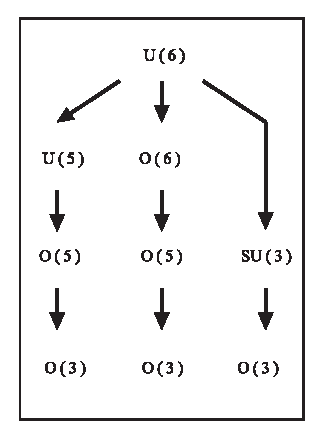
\includegraphics[scale=.65]{figure}
%
% If not, use
%\picplace{5cm}{2cm} % Give the correct figure height and width in cm
%
\caption{Please write your figure caption here}
\label{fig:A1}       % Give a unique label
\end{figure}

% For tables use
%
\begin{table}
\caption{Please write your table caption here}
\label{tab:A1}       % Give a unique label
%
% For LaTeX tables use
%
\begin{tabular}{p{2cm}p{2.4cm}p{2cm}p{4.9cm}}
\hline\noalign{\smallskip}
Classes & Subclass & Length & Action Mechanism  \\
\noalign{\smallskip}\hline\noalign{\smallskip}
Translation & mRNA$^a$  & 22 (19--25) & Translation repression, mRNA cleavage\\
Translation & mRNA cleavage & 21 & mRNA cleavage\\
Translation & mRNA  & 21--22 & mRNA cleavage\\
Translation & mRNA  & 24--26 & Histone and DNA Modification\\
\noalign{\smallskip}\hline\noalign{\smallskip}
\end{tabular}
$^a$ Table foot note (with superscript)
\end{table}
%


\backmatter%%%%%%%%%%%%%%%%%%%%%%%%%%%%%%%%%%%%%%%%%%%%%%%%%%%%%%%
%%%%%%%%%%%%%%%%%%%%%%acronym.tex%%%%%%%%%%%%%%%%%%%%%%%%%%%%%%%%%%%%%%%%%
% sample list of acronyms
%
% Use this file as a template for your own input.
%
%%%%%%%%%%%%%%%%%%%%%%%% Springer %%%%%%%%%%%%%%%%%%%%%%%%%%

\Extrachap{Glossary}


Use the template \emph{glossary.tex} together with the Springer document class SVMono (monograph-type books) or SVMult (edited books) to style your glossary\index{glossary} in the Springer layout.


\runinhead{glossary term} Write here the description of the glossary term. Write here the description of the glossary term. Write here the description of the glossary term.

\runinhead{glossary term} Write here the description of the glossary term. Write here the description of the glossary term. Write here the description of the glossary term.

\runinhead{glossary term} Write here the description of the glossary term. Write here the description of the glossary term. Write here the description of the glossary term.

\runinhead{glossary term} Write here the description of the glossary term. Write here the description of the glossary term. Write here the description of the glossary term.

\runinhead{glossary term} Write here the description of the glossary term. Write here the description of the glossary term. Write here the description of the glossary term.

\Extrachap{Solutions}

\section*{Problems of Chapter~\ref{intro}}

\begin{sol}{prob1}
The solution\index{problems}\index{solutions} is revealed here.
\end{sol}


\begin{sol}{prob2}
\textbf{Problem Heading}\\
(a) The solution of first part is revealed here.\\
(b) The solution of second part is revealed here.
\end{sol}


\printindex

%%%%%%%%%%%%%%%%%%%%%%%%%%%%%%%%%%%%%%%%%%%%%%%%%%%%%%%%%%%%%%%%%%%%%%

\end{document}





